\documentclass[12pt,a4j]{jsreport}
\usepackage[dvipdfmx]{graphicx}
\usepackage[dvipdfmx]{xcolor}
\usepackage[deluxe,uplatex]{otf}  % 日本語用フォントサポート
\usepackage{caption}  % キャプションの整形
\usepackage{comment} 
\usepackage{multirow}
\usepackage[numbers,sort&compress]{natbib}
\usepackage{tcolorbox}
\tcbuselibrary{breakable}
\usepackage{minted}
\usepackage{capt-of}


\setcitestyle{numbers,square,comma}

% 各章のタイトルが改行されてしまう現象が発生したので追記
\usepackage{titlesec}
\titleformat{\chapter}[hang]
  {\huge\bfseries}
  {第\thechapter{}章\ }
  {0pt}
  {}

\begin{document}

% タイトルページ
\thispagestyle{empty}
\begin{center}
修士論文\\% どちらか一方を消してください.
\vfill
指導現場で生じるインタラクションに基づいた\\
大規模言語モデルによる熟練者の知識構造化支援\\
ー 社交ダンスを例として ー\\
\vfill
石井 遼太郎\\
\vfill
主指導教員 西村 拓一\\
\vfill
北陸先端科学技術大学院大学\\
先端科学技術研究科\\
(知識科学)\\ %取得希望学位
\vfill
令和7年3月\\ % 学位授与年月
\vfill
\end{center}

\clearpage
\thispagestyle{plain}

% Abstract
\centerline{Abstract}
This study aims to establish a system for extracting and sharing the knowledge of skilled practitioners in a natural context within the field of skill transfer. To achieve this goal, we propose a novel method combining dialogue collection in instructional settings with knowledge extraction support using Large Language Models (LLMs), and verify its effectiveness through empirical experiments in ballroom dancing.

The empirical study analyzed five weeks of practical data from two instructors and thirteen learners. The results showed that 76\% of instructional comments contained previously unincorporated elements, demonstrating the possibility of extracting new knowledge elements through natural interactions in daily instructional activities. Furthermore, LLMs demonstrated high accuracy (F-value: 0.928) in extracting unincorporated elements, confirming their contribution to systematic knowledge organization.

A significant finding was the discovery of the dual nature of knowledge structure in ballroom dancing: the aspect of chronological sequence of movements and the underlying theoretical knowledge. Based on this finding, we propose two classification frameworks: a four-layer structure for understanding skills and a classification based on execution layer characteristics. Drawing from these frameworks, we propose a new knowledge representation method that separately describes chronological movements in a single layer and represents underlying theoretical knowledge as purpose-oriented knowledge. This approach has potential applications not only in ballroom dancing but also in other physical skill domains with similar characteristics.
\clearpage

% 目次
\tableofcontents
\clearpage

% 図目次と表目次
\listoffigures
\clearpage
\listoftables
\clearpage

% ページ番号をリセット
\setcounter{page}{1}

% 第1章{序論}
\chapter{はじめに}
 熟練技能者の高齢化や後継者不足が深刻化する中, 長年培われてきた技能の存続が危ぶまれている. 労働政策研究・研修機構の調査によれば, 2020年の時点で調査対象の企業のうち技能継承を重要だと考えている企業が95\%に達している. しかしながら, 技能者の人材育成や能力開発の取り組みがうまくいっていると認識している企業は約55\%にとどまっている\cite{JILPT2020}. このような状況から, 技能伝承を実現するための取り組みが求められている. ここで技能について考えてみると, ある目的を達成するためには, それをどのように行うかを理解していること(わかる)と, 実際に行えること(できる)の両方が必要となる. このことから本研究では, 技能を, 理解と, それを実行に移すための実践的能力から構成される実践的な能力として定義する. なお, 実践的能力には身体的な動作制御から認知的な処理能力まで含まれる. このような技能を次世代に伝えていく営みが技能伝承である.\\
 技能伝承を実現するためには, 熟練技能者の持つ理解を明確化し, それを体系的に整理した上で, 育成対象の人材が実践を通じて習得し, さらにその経験を通じて新たな気づきを得るという循環的なプロセスが重要である. 本研究では, このような技能の理解に関わる部分を「知識」と表現する. これには明示的に説明可能な作業手順から, 経験に基づく暗黙的な判断基準まで含まれる.\\
 この循環的なプロセスの中でも, 熟練技能者の持つ知識を明確化し体系的に整理する段階は, その後の技能伝承活動の基盤となる重要な要素である. この知識抽出の方法について, Tatianaらは研究者と熟練技能者の関係性に基づいて, 研究者主導型, 協働型, 熟練技能者主導型の3つに分類している\cite{Tatiana2012}. このうち熟練技能者主導型(Expert-leading)は, 技能伝承を必要とする現場に比べて研究者の数が限られている現状を考慮すると, 持続可能性の観点で優位性を持つと考えられる.\\
 「Expert-leading」に分類される知識抽出手法として, 西村らが提案した"知識発現"\cite{Nishimura2017}がある. この手法ではまず, 既存のマニュアルから手順を構造的に記述したプロセス知識を作成する. 次に, 作成したプロセス知識をベースとして現場の従業員が具体的な事例の紐付けと議論を行うことで, プロセス知識を改良しながら知識を抽出していく. この手法は現場が自律的に知識を抽出できる一方で, 未経験者の理解, 知識記述の限界, 記述漏れ, ワークショップ形式に起因する時間的制約, 情報システム化に向けた課題など, いくつかの実践的な課題が存在する.\\
 本研究の目的は、技能伝承の現場において、熟練技能者の持つ知識を継続的に抽出・共有できる持続可能な仕組みを確立することである. 本研究では,西村らの研究\cite{Nishimura2017}で用いられたプロセス知識をベースにしながら, 技能伝承の現場における指導者と学習者の対話ログ,多量なオープンデータから構成された大規模言語モデル(LLM)を組み合わせることで,より実践的な知識の抽出手法を提案する. 具体的には技能の指導現場に着目する. まず, 技能継承の対象となる動作のベースとなる知識モデル(プロセス知識)を作成しておく. 次に, 指導現場における, 熟練技能者, すなわち指導者と学習者のやりとりを収集する. 次に指導現場で収集した情報をLLMが解析し既存のプロセス知識の改良点を生成し提案する. そしてLLMによる改良提案を受けた指導者が最終的にプロセス知識を改良する.\\
 これらの要素の組み合わせにより, 先行研究で指摘された未経験者の理解に関する課題や知識記述の限界, 記述漏れのリスクなどに対して, 複合的なアプローチが可能となる. 例えば, 指導現場での対話収集により未経験者の視点を取り入れることができ, またLLMの活用により収集した対話から新たな知見を抽出することで, 知識記述の幅を広げることができる.\\
 本研究では, 社交ダンスの指導現場を対象として提案手法の有効性を検証した. 具体的には, ダンススタジオの指導者2名と学習者13名の協力のもと, 3週間にわたってオンライン指導システムを用いた指導内容の収集を行った. また, 収集したデータをLLMに解析させ, 生成された改良点の提案について指導者から評価を得た. さらに, これらの結果を踏まえて指導者がプロセス知識を改良する過程についても検証を行った.\\
 本稿は以下のように構成される. 第2章では関連研究について述べ, 本研究の立場を明らかにする. 第3章では提案手法について, その理論的背景と具体的な実現方法を詳述する. 第4章では実験システムの構築とそのための予備検証について説明する. 第5章ではダンススタジオでの実証実験とその結果について述べる. 第6章では考察を行い, 最後に第7章でまとめと今後の展望を述べる.\\




% 第2章{先行研究・関連研究}
\chapter{関連研究}
\section{"知識"とその抽出に関する研究}
- 対象とする「知識」のスコーピング -\\
ポランニーは「我々は語れる以上のことを知っている(We know more than we can tell)」と述べ, 本質的に言語化できない知識の存在を指摘した\cite{Polanyi1966}. このような言語化できない知識は, 技能伝承において特に重要な課題となる.

野中・竹内が提唱したSECIモデルでは, 知識を暗黙知と形式知という2つの形態で捉え, それらの相互変換による知識創造のプロセスを説明している\cite{Nonaka1996}. このモデルでは, 暗黙知から形式知への変換(表出化), 形式知同士の組み合わせ(連結化), 形式知の実践を通じた暗黙知化(内面化), そして経験の共有による暗黙知の伝達(共同化)という4つのフェーズを通じて知識が発展していくとされる.

本研究では, 技能伝承を持続的に実現可能なものとするため, まず形式知化が可能な領域において知識抽出の手法を確立することを目指す. 本質的に言語化できない知識は, 定量的なデータ計測による分析や, 直接的な経験の共有による伝達が必要となるが, 形式知化が可能な知識は, 言語や図表による表現を通じて時間や場所の制約を超えた伝達が可能となる. 具体的には, 熟練技能者の持つ暗黙知を形式知として明示化し(表出化), それを体系的に整理する(連結化)プロセスに着目する. これらのプロセスは, その後の技能習得や新たな知識創造の土台となる.\\

- 抽出手法の分類 -\\
Tatianaらは, SECIモデルのような知識の循環的プロセスにおける「知識を明確化し, 体系的に整理する」段階に着目し, 知識抽出手法を研究者と熟練技能者の関係性に基づいて3つに分類している\cite{Tatiana2012}. 「Analyst-leading」は, 研究者が主体となって熟練技能者から知識を引き出す手法である. 具体的には, 研究者が熟練技能者にインタビューやアンケートを行うことで知識を抽出する. この手法は熟練技能者の明示的な知識を効率よく引き出せる一方で, 抽出できる知識が表層的であったり, 効果的なインタビューのためには長年の訓練と経験が必要であるといった課題がある. 「Expert-Analyst Collaborating」は, 研究者と熟練技能者が協働して知識を抽出する手法である. 具体的には, ロールプレイングゲームやバーバルプロトコルなどを通じて両者が体験を共有しながら知識を抽出する. この手法は熟練技能者が持つ本質的な知識を抽出できる一方で, 体験共有の場の準備や, 研究者が現場の専門知識を理解する必要があるなど, 多大な労力を必要とする. 「Expert-leading」は, 熟練技能者が主体となって自ら知識を抽出する手法である. 具体的には, ストーリーテリングやブレインストーミングなどを通じて知識を抽出する. この手法は研究者の介入コストが低い一方で, 抽出された知識が体系的にまとまりづらく, また熟練技能者自身が知識の言語化に苦労するという課題がある.\\

- 知識発現 -\\
このうちExpert-leadingに分類される代表的な手法として, 第1章でも述べた, 西村らの"知識発現"\cite{Nishimura2017}がある. この手法では, プロセス知識をベースとして現場の従業員が具体的な事例の紐付けと議論を行うことで, 知識を抽出していく. しかし, 以下のような実践的な課題が明らかになっている.
\begin{enumerate}
    \item 未経験者の理解に関する課題\\
    構造化されたプロセス知識の背景知識を持たない場合, その内容を読み解くことが困難である可能性がアンケート結果から示唆されている.\\
    
    \item 記述できる知識の限界に関する課題\\
    ワークショップ参加者間の議論のみで知識を抽出するため, 参加者が意識的に想起できる知識の総量以上のものは記述できず, 熟練技能者が無意識のうちに実践している暗黙的な知識を十分に引き出せない可能性がアンケート結果から示唆されている.\\
    
    \item 記述漏れに関する課題\\
    系統立てた記述により自然言語の自由記述に比べて記述漏れに気づきやすいものの, 完全な解決には至っていない.\\
    
    \item ワークショップ形式に起因する課題\\
    ワークショップという限られた時間と場所での議論では, 実際の業務で直面する様々な状況を網羅的に想起することが難しく, また参加者の時間的負担も大きいため, 継続的な知識抽出活動の実施が困難である.\\
    
    \item 情報システム化に向けた課題\\
    知識抽出活動を効率的に実施し継続的に改善していくためには情報システムによる支援が必要であるが, 事例とプロセス知識との関連性を直感的に表現できるUIの実現や, より効果的な知識想起を促す知識モデルの設計など, 実用化に向けた技術的な課題が残されている.\\
\end{enumerate}

これらの課題に対し, 本研究では指導現場に着目することとLLMを活用することで複合的な解決アプローチを提案する. 

まず, 未経験者の理解に関する課題に対しては, 指導現場での学習者からの質問や反応を通じて, 未経験者が理解しづらい点を直接的に把握できる. またLLMが収集した対話から理解を妨げる要因を分析し, より理解しやすい形での知識の表現を提案することができる.

知識記述の限界に対しては, 指導現場での予期せぬ質問が熟練技能者の無意識の知識を引き出すきっかけとなり, さらにLLMが収集した対話から新たな知見を抽出することで, 知識記述の幅を広げることができる. 

記述漏れの課題に対しては, LLMが収集された対話を分析することで, 体系的な観点から漏れている知識を指摘できる可能性がある. また, 指導現場という実践の場での継続的な対話収集により, 様々な状況における知識を網羅的に収集できる.

ワークショップ形式に起因する課題に対しては, 指導現場という日常的な文脈で知識抽出を行うことで, 時間的制約や想起の困難さを軽減できる. 

最後に情報システム化に向けた課題に対しては, LLMを活用することで, 収集した対話から知識モデルの改良点を自動的に提案できる可能性がある.\\

- その場その場での記録 -\\
知識抽出に関する他の研究として, 内平ら\cite{Uchihira2022}は, 日常的なつぶやきを音声情報として収集し知識を獲得する手法を提案している. この手法の特徴は, 業務中の気づきや閃きをその場で自然に収集できる点にあり, 知識抽出をより日常的な活動として実現している.  

本研究も同様に, 指導現場という自然な文脈での即時的な知識抽出を目指すが, さらにLLMを活用することで収集した知識の分析と体系化を行う点に新規性がある. また, 内平らの提案する手法と本研究は, どちらも日常的な活動の中で自然に知識を収集するという点で共通しており, これらを組み合わせることでより包括的な知識抽出システムを実現できる可能性がある. 例えば, 指導現場での気づきを音声情報として収集しながら, 指導内容をLLMで分析・体系化するといった相補的な活用が考えられる.\\



\section{指導現場に着目した研究}
これまで指導現場で生じるインタラクションに関する研究も行われてきた.Moore\cite{Moore1989}は, 教育における相互作用を学習者-コンテンツ間, 学習者-指導者間, 学習者間の3つに分類し, 特に学習者-指導者間の相互作用において, 指導者は自身の経験に基づいて学習者の理解を促進させることを指摘している.この知見は, 指導現場における相互作用が, 熟練者の持つ知識を表出させる機会となる可能性を示唆している.

広瀬・深澤\cite{Hirose2018}は, 指導における言語使用について, 科学言語(直示的な表現)とわざ言語(比喩的な表現)という観点から理論的な分析を行っている.特に, 指導場面における対話的状況では, 発話者が想定する「現実」を学習者と共有することの重要性を指摘している.ただし, この研究は理論的な枠組みの提示に留まっており, 実際の指導現場での言語使用を通じた知識抽出については検討されていない.

佐伯ら\cite{Saeki2017}は, 指導者の成長プロセスに着目し, 経験と省察を通じて指導力が向上していく過程を分析している.この研究は指導者の経験が言語化される過程を示唆しているが, 指導現場でのインタラクションを通じた知識抽出という観点からの分析は行われていない.

これらの先行研究は, 指導者の知識や経験に関する重要な知見を提供している一方で, 実際の指導現場でのインタラクションを通じて熟練者の知識を抽出する方法については十分な検討がなされていない.特に, 学習者との相互作用の中で熟練者がどのように自身の知識を表出させ, それをどのように抽出できるのかについては, さらなる検討が必要である.
本研究では, これまでの研究で十分に検討されてこなかった指導現場でのインタラクションに着目し, そこから熟練者の持つ知識を抽出する方法を明らかにすることを目指す.\\



\section{LLMを活用したナレッジマネジメントシステムの研究}
近年, LLMの発展により様々な知的活動への活用が研究されている. 大きく分けると,(1)創造性支援ツール(CST)としての活用,(2)LLMの性能向上に関する研究, (3)知識ベース構築への活用という3つの方向性がある.

創造性支援ツール(CST)としての活用について, 田中らはマルチエージェントのアプローチを提案している\cite{Tanaka2024}. この手法では, 異なる役割を持つLLMエージェントが対話的にアイデアを生成することで, 単一のエージェントでは得られない多様な発想を引き出すことができる. また, 尾崎らはLLMに反論文を生成させることで, 議論における批判的思考を補完する手法を提案している\cite{Ozaki2024}. これらの研究から, LLMを適切に活用することで発散的思考や収束的思考の支援, さらには認知バイアスの軽減などの効果が期待できることが示唆されている.

LLMの性能向上に関して, WelzらやLewisらは外部知識ベースを活用することで, LLMが生成するコンテンツの事実性を向上させる手法を提案している\cite{Welz2024, Lewis2020}. これらの研究は, LLMと既存の構造化された知識を組み合わせることの有効性を示している.

知識ベース構築への活用においては, ShenとLin\cite{Shen2024}は, LLMを搭載した個人用知識アシスタント(K-assistant)を提案している. このシステムでは, 自然言語処理, 理解, 推論の機能を組み合わせることで, 実践コミュニティ(CoP)のメンバー間の知識活動を支援する.特に, 暗黙知から形式知への変換プロセスを促進する点で, 従来の知識抽出手法とは異なるアプローチを取っている.また, 鵜飼らはLLMを使用して知識ベースそのものを構築する手法を提案している\cite{Ukai2023}が, 現状のLLMの性能では知識ベースをゼロから生成することは困難であり, 人間の専門知識による検証や修正が必要とされている.

これらの先行研究に対し, 本研究の新規性は以下の点にある.第一に, 従来研究の多くがLLMの性能向上や汎用的な知識ベースの構築を目指していたのに対し, 本研究は熟練技能者特有の知識抽出に焦点を当てている.第二に, LLMを知識抽出の補助ツールとして位置づけ, 人間とLLMが相互に補完し合いながら知識を抽出・構造化するプロセスを提案している. 特に、指導現場での対話分析を通じて、熟練者が持つまだ言語化されていない知識を、LLMを活用して体系的に抽出・整理する点は、これまでにない新しいアプローチである。

% 第3章{提案手法}
\chapter{提案手法}
\section{提案手法の概要}
本研究は, 技能伝承の現場において, 熟練技能者の持つ知識を継続的に抽出・共有できる持続可能な仕組みを確立することを目指す. これは, SECIモデルにおける「表出化」と「連結化」のプロセスに焦点を当て, 特に形式知化が可能な領域での知識抽出手法の確立を意味する.

知識発現\cite{Nishimura2017}をはじめとする従来の知識抽出手法では, 日常的な活動として知識抽出を継続的に行うことが困難であった. 本研究ではこの課題に対し, 技能の指導現場に着目し, LLMを活用した複合的なアプローチを提案する. 

具体的には, 以下の3つの要素を組み合わせることで, 日常的な知識抽出の仕組みを実現する.
\begin{enumerate}
    \item 知識の基盤 : 西村らの研究で提案されたプロセス知識の考え方を基礎とし, 知識工学の手法を用いて体系的に整理する
    \item 指導現場での対話収集 : 指導者と学習者の自然なやりとりから, まだ言語化されていない知識を抽出する
    \item LLMを用いた支援 : 収集した対話を分析し, 基盤となる知識の改良点を提案する
\end{enumerate}

これにより, 日常的な指導活動の中で知識を抽出しながら, LLMによる分析支援のもと, 熟練技能者が知識を整理・構造化することが可能となる. なおこれ以降, 本稿では技能伝承の文脈において熟練技能者を指導者と表記する. 以下, 提案手法の詳細について説明する.

\section{提案手法の仕組み}
本提案手法の全体像を図\ref{fig1}に示す. 先述の通り, 指導現場での日常的なインタラクションを通じて知識を抽出・構造化する.

まず, 指導対象となる技能についてのベースとなるプロセス知識を作成する. これは教科書や既存のマニュアルなどの形式知をもとに, 指導者の協力を得ながら構築する. このベースとなるプロセス知識は, 以降の知識抽出・構造化の土台となる. 

次に, 指導者の発言を自動的にロギングする. これには指導内容だけでなく, 学習者の理解度に応じた補足説明や, 予期せぬ質問への応答なども含まれる. 同様に, 学習者からの質問や感想といった応答も自動的に記録する. これらの対話ログは, 指導現場での暗黙的な知識のやり取りを捉える重要な情報源となる. 

収集された対話ログは, 既存のプロセス知識と併せてLLMによって解析される. LLMは対話の文脈を理解し, 現在のプロセス知識に不足している要素や, より詳細な説明が必要な箇所を特定する. そして, これらの分析結果に基づいて, プロセス知識の改良点を指導者に提案する. 

指導者はLLMからの提案を参考に, プロセス知識を改良することができる. ただし, この改良はLLMからの提案に限定されず, 指導者が日々の指導の中で気づいた点があれば, 随時プロセス知識を更新することも可能である. 

一方, 学習者もプロセス知識を参照することで, 指導内容への理解を深めることができる. これは単なる知識の参照に留まらず, 学習者からの新たな質問や気づきを生み出すきっかけともなり, さらなる知識の抽出・構造化のサイクルにつながっていく. 

このように, 提案手法は指導現場での自然なやりとりを起点として, LLMによる支援のもと, 継続的に知識を抽出・構造化していく仕組みを実現する. 

\begin{figure}[htbp]
    \centering
    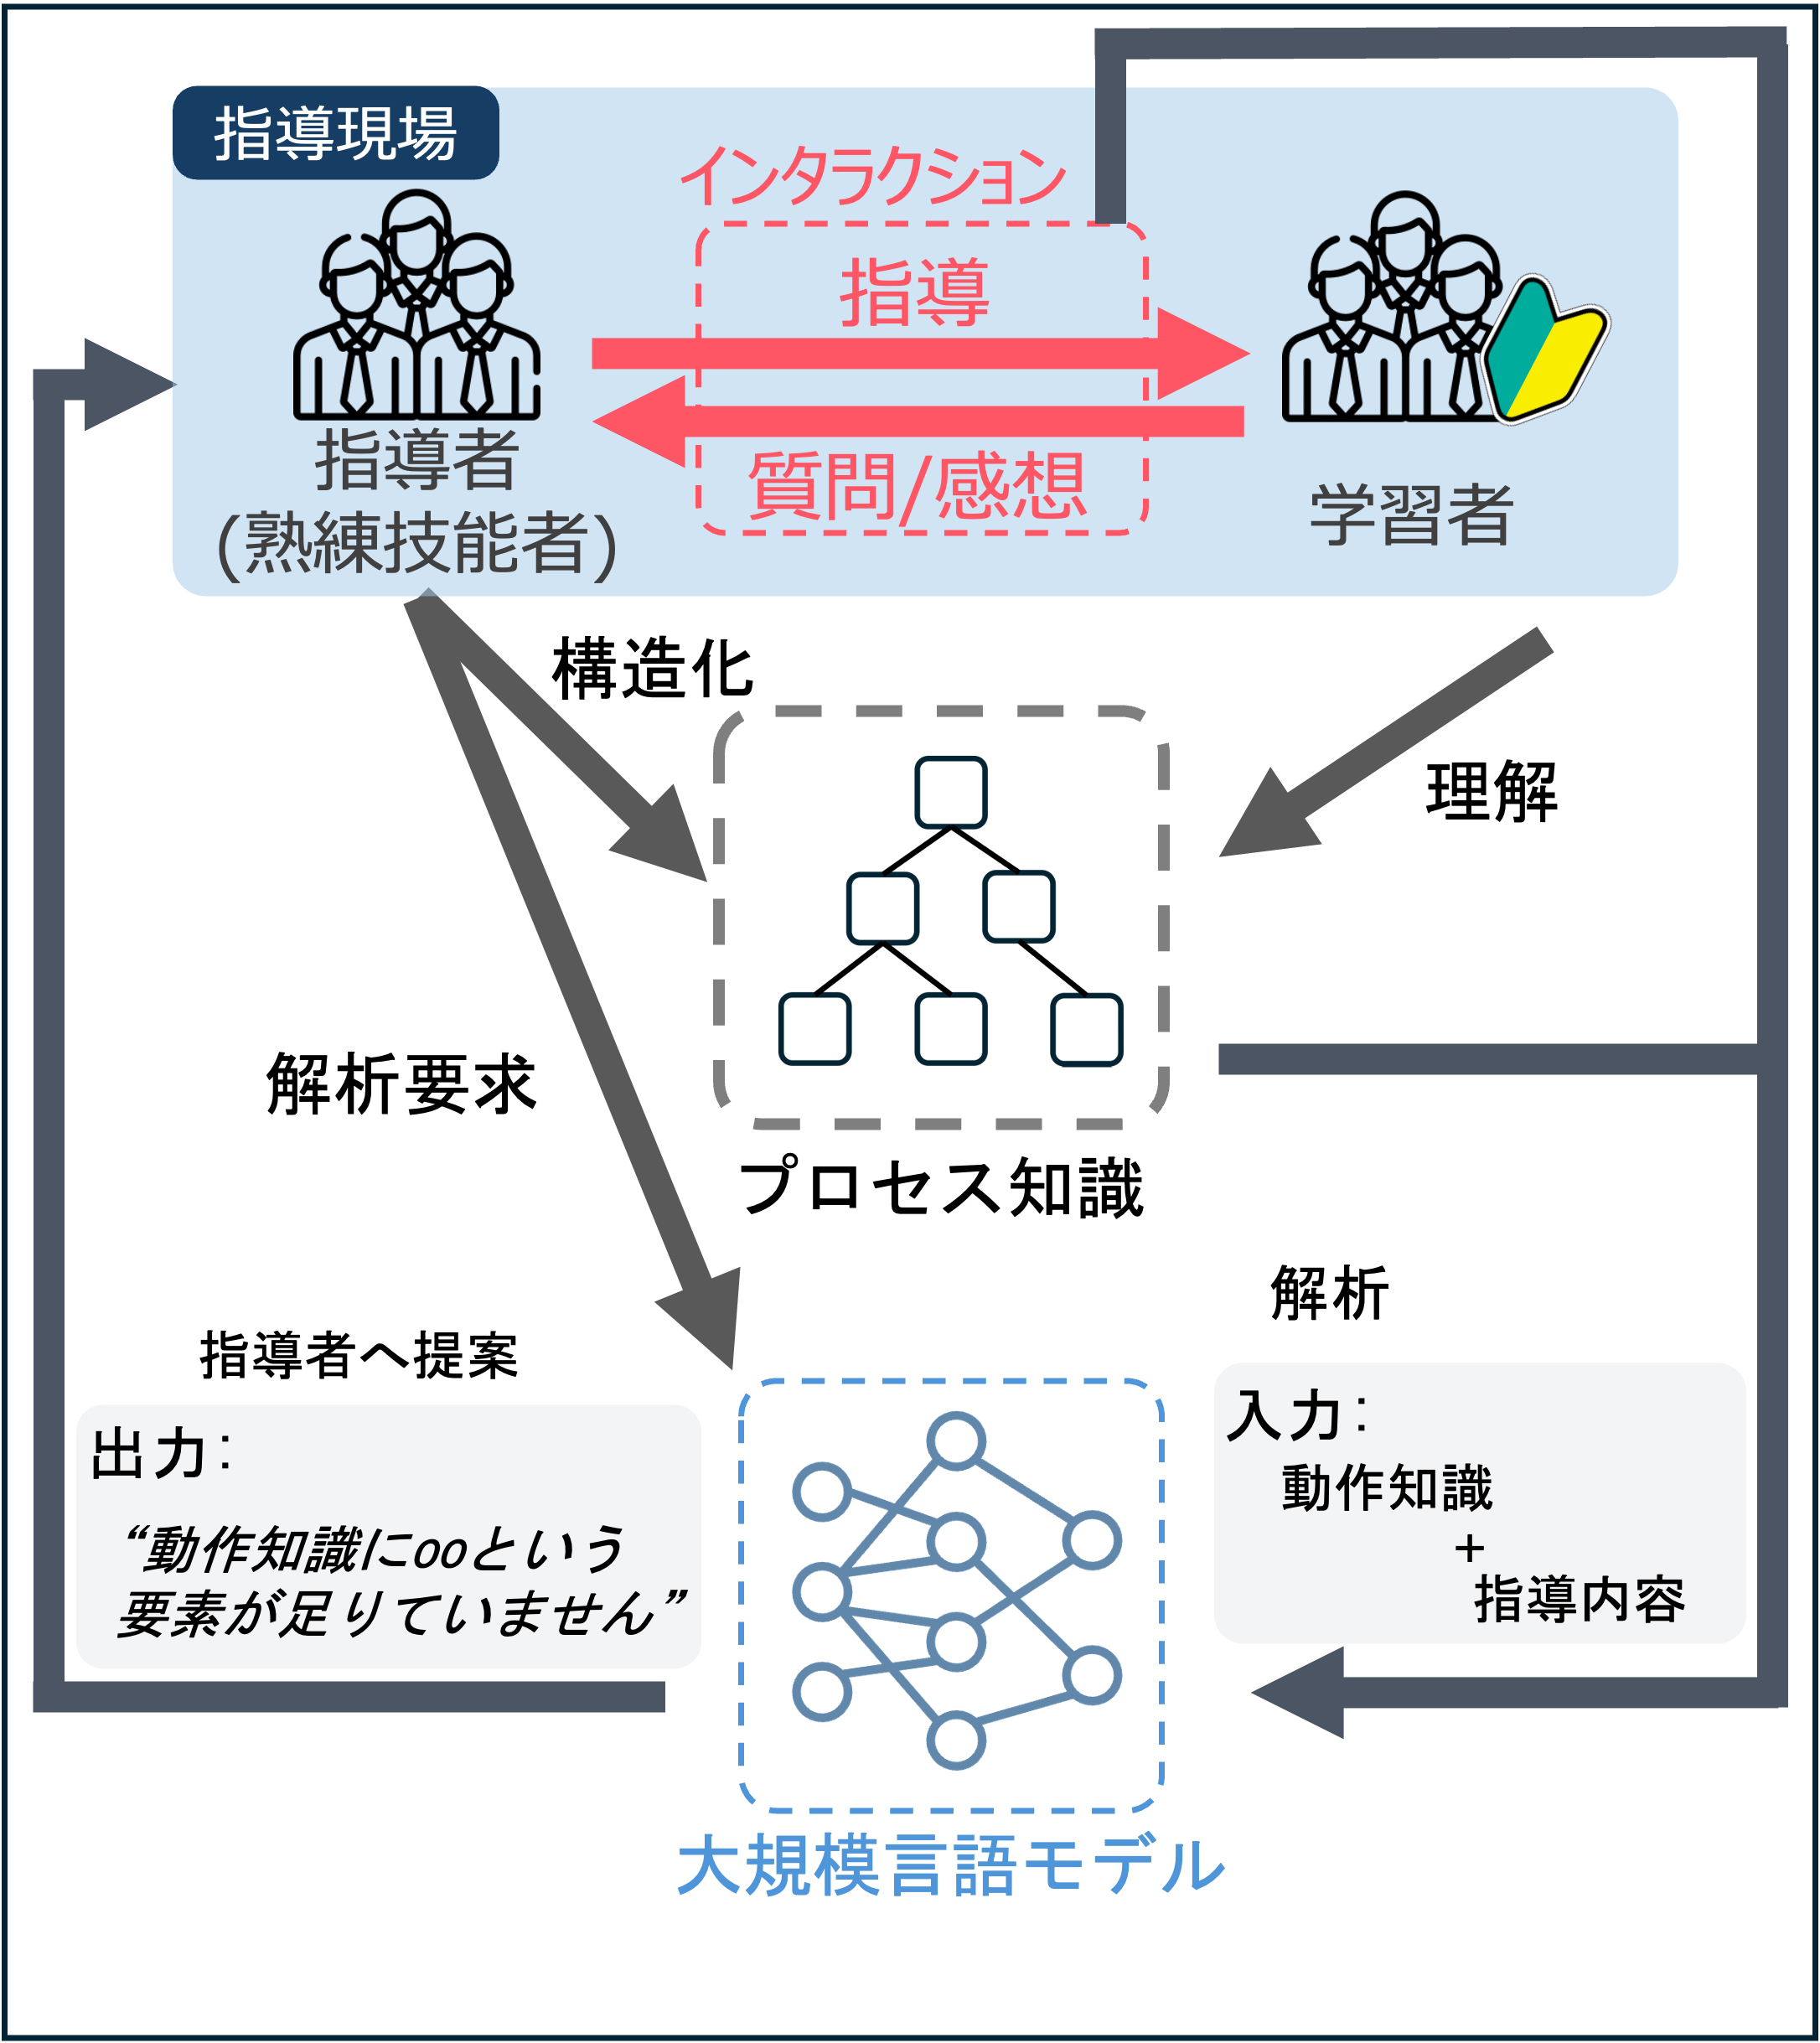
\includegraphics[width=1.0\linewidth]{./image/overview_2.png}
    \caption{提案手法の全体像}
    \label{fig1}
\end{figure}


% 第4章{実験}
\chapter{実験の準備}
提案手法の有効性を検証するため, 実験環境の整備を行った. 本章では, プロセス知識の記述方法の選定から, 指導現場でのインタラクション収集の仕組み, LLMを用いた知識抽出支援機能の開発に至るまでの準備について説明する. 

\section{プロセス知識の記述方法}
本研究では, 西村らが提案したCHARM (Convincing Human Action Rationalized Model) \cite{Nishimura2008, Nishimura2015}を採用する. これは, 人間の行為とその目的を体系的に表現するためのモデルであり, 機械工学分野で用いられる機能分解木の考え方を応用して開発された.

CHARMは,ある行為をそれを達成するために必要な行為の系列に分解することで,行為間の目的達成関係を記述する. 具体的には,上位層の行為ノードを達成するために下位層の行為ノードを実行するという階層構造として表現される. 各ノードには行為の実行者や実行条件などのプロパティを付与することができ,これにより各行為の目的の把握を容易にする. また,同一の目的に対して複数の実現手段が存在する場合,それらを並列的に記述することで,状況に応じた手段の選択を支援する. 

CHARMの重要な特徴として, 形式知化された知識と暗黙知の橋渡しを支援する点が挙げられる. 具体的には, 行為とその目的の関係性を明示することで, 「なぜその行為が必要か」という理由付けを含めた知識表現を実現する. これにより, 単なる手順の羅列ではなく, 状況に応じた柔軟な対応を可能にする知識構造を構築できる.

実際に, 看護業務における技能伝承の現場での実証実験を通じてCHARMの有効性が確認されている. 特に, 暗黙知の抽出や組織間での知識共有においてその有用性が示されている. これは, CHARMが持つ目的指向的な知識表現と問題-対策の構造化という特徴が実践的な知識管理に適していることを示唆している.

本研究では, CHARMを計算機上で扱うためにリレーショナルデータベース(RDB)を構築した(図\ref{fig2}). 実装には木構造をRDBで表現するための閉包テーブルというデータベース構造を採用した. また, 後述する各種システムからアクセス可能なエンドポイントを設けてある.

CHARMに基づいて作成したプロセス知識の例を図\ref{fig3}に示す. これは社交ダンスのナチュラルターンに関するプロセス知識である.

\begin{figure}[htbp]
    \centering
    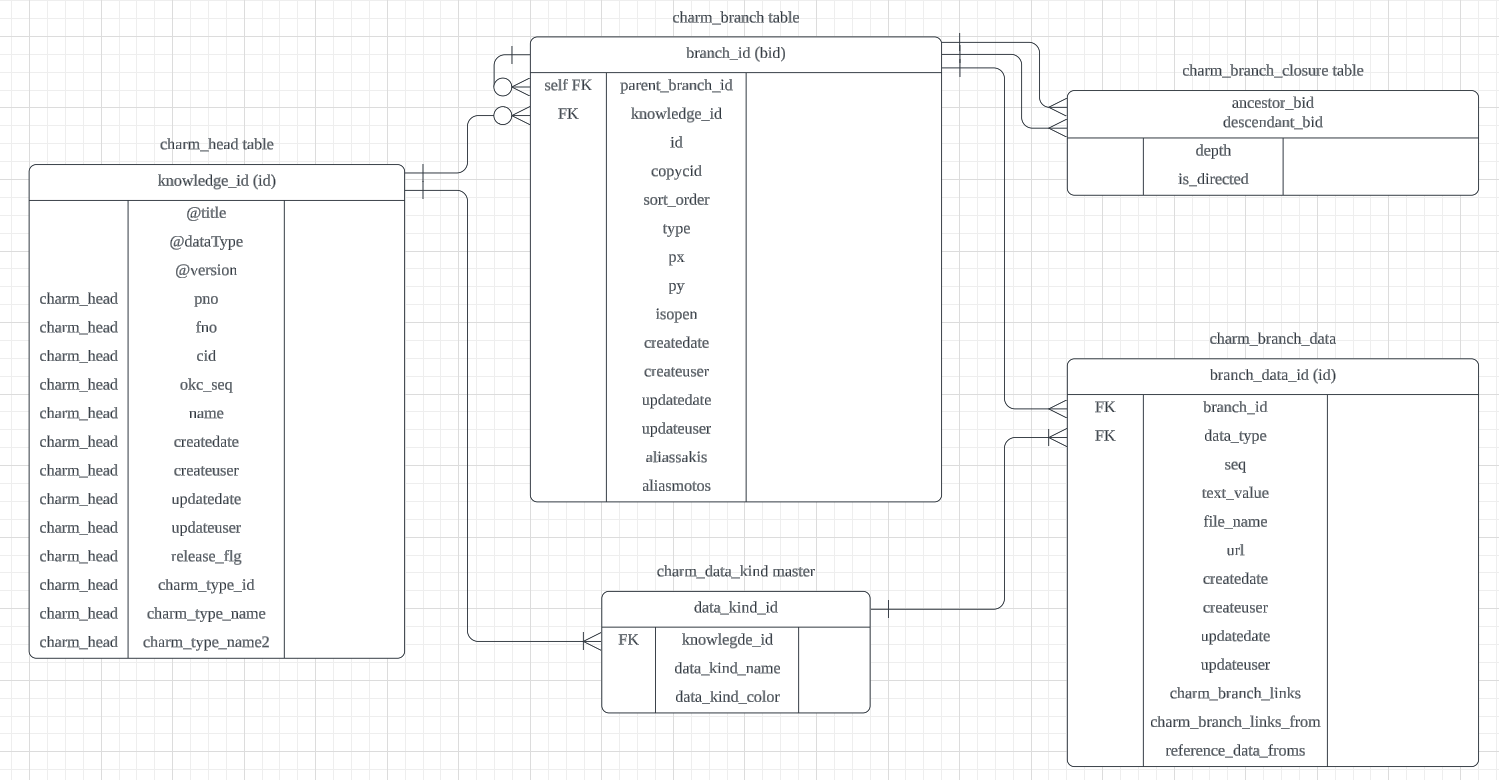
\includegraphics[width=1.0\linewidth]{./image/charm_database.png}
    \caption{CHARMのリレーショナルデータベース表現}
    \label{fig2}
\end{figure}

\begin{figure}[htbp]
    \centering
    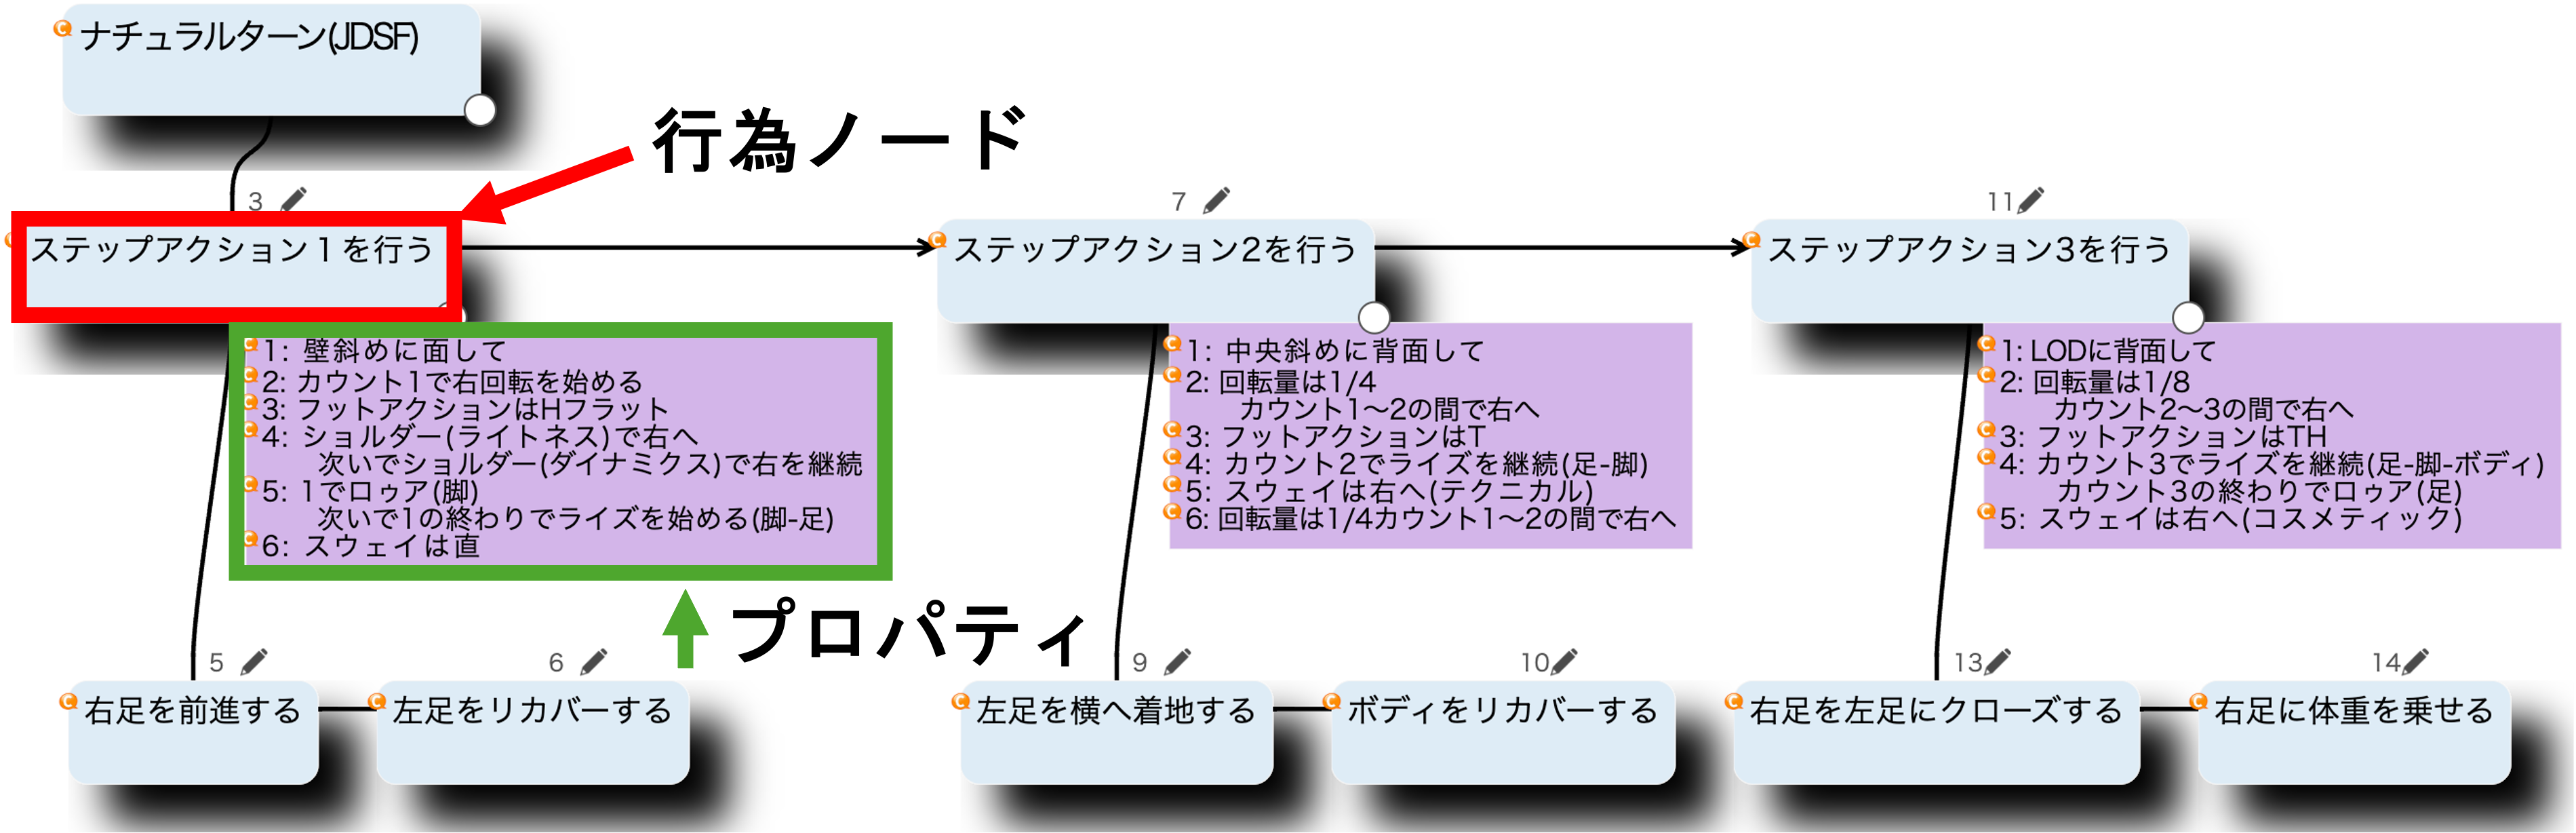
\includegraphics[width=1.0\linewidth]{./image/charm_natural_turn.png}
    \caption{CHARMに基づいて記述した社交ダンスのナチュラルターンに関するプロセス知識}
    \label{fig3}
\end{figure}



\section{指導現場のインタラクションを収集するシステムの開発}
本研究では、指導者と学習者のインタラクションを効果的に収集するため、加藤らが開発した知識連携アノテーションシステム\cite{Kato2023}を拡張する。このシステムは、オンライン動画添削システムにCHARMを統合したもので、学習者の動作動画に対して指導者がプロセス知識内の行為ノードと紐付けながらコメントを付与することができる。本研究では、このシステムに双方向のコミュニケーション機能を追加し、付与されたコメントに対して指導者と学習者が対話的にやりとりできる仕組みを実現した。

システムのデモ画面を図\ref{fig4}, 図\ref{fig5}に示す. 図\ref{fig4}は既存の知識連携アノテーションシステムの画面である. この画面では, アノテーションの表示時間, 動画内での表示座標, プロセス知識内の関連する行為ノード, およびアノテーションテキストを入力することができる. 「ok」ボタンを押すとアノテーションがデータベースに登録され, 動画内に表示される.

図\ref{fig5}は本研究で新たに追加した双方向コミュニケーション機能の画面である. 画面上部のコメント一覧には図\ref{fig4}で追加したアノテーションが表示され, いずれかのアノテーションをクリックするとその下にチャット画面が展開される. このチャット画面を通じて, 指導者と学習者は選択したアノテーションに関する質問や感想などを交換することができる. なお, 図\ref{fig4}と図\ref{fig5}の画面間の遷移は, 画面最上部に配置した「コメント入力画面」および「チャット画面」ボタンから行う.

システムの実装には, PythonのWebアプリケーションフレームワークであるDjangoを使用した. また, システムの信頼性と保守性を考慮し, Webサーバーとは別個にMySQLデータベースサーバを設置してデータを管理している.

\begin{figure}[htbp]
    \centering
    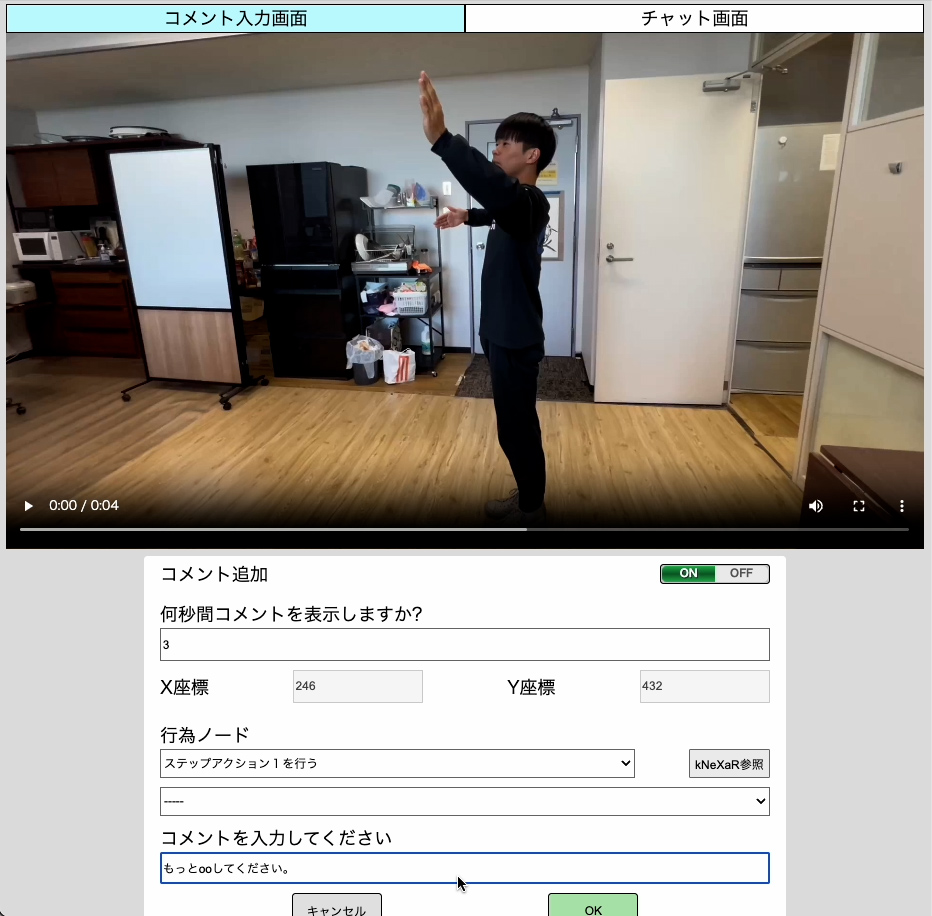
\includegraphics[width=1.0\linewidth]{./image/demo_annotation.jpg}
    \caption{アノテーション画面}
    \label{fig4}
\end{figure}

\begin{figure}[htbp]
    \centering
    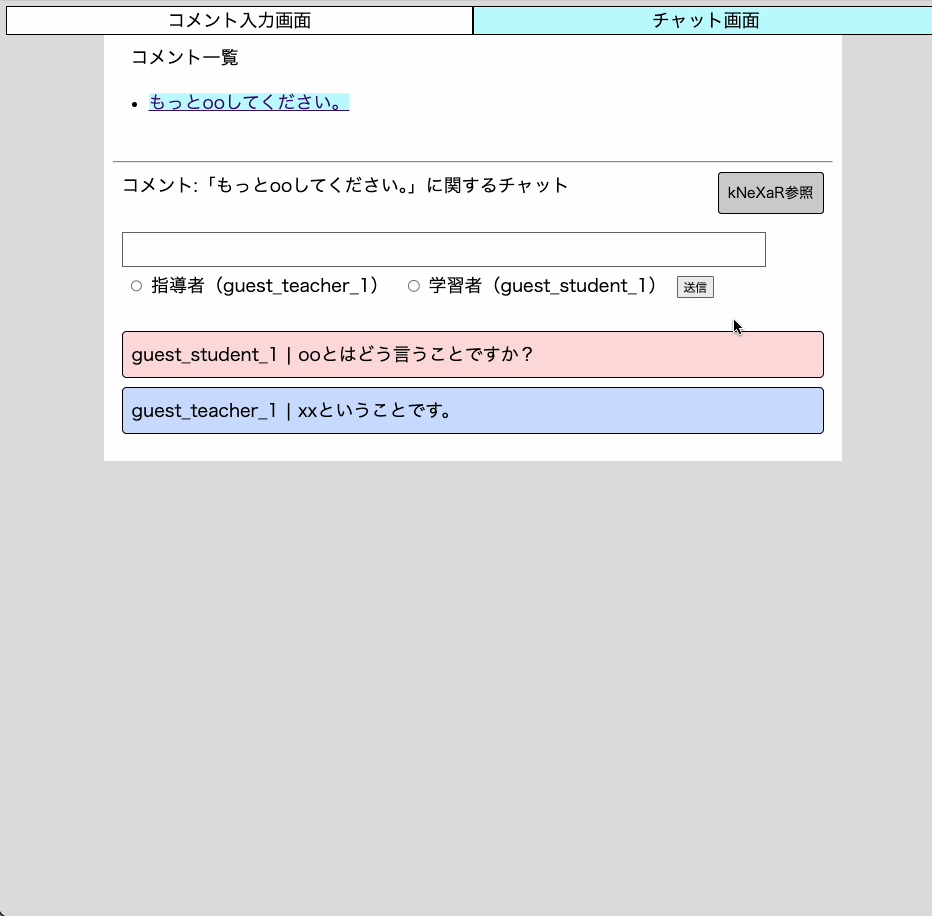
\includegraphics[width=1.0\linewidth]{./image/demo_chat.jpg}
    \caption{やりとり画面}
    \label{fig5}
\end{figure}



\section{LLMを用いた知識抽出支援機能の開発}
LLMを知識抽出の支援ツールとして活用するために, モデルの選定から本研究での利用可能性の検証, そしてシステムへの実装までを段階的に行った. 本節では, まずLLMの選定とその理由について述べ, 次に知識抽出タスクにおける利用可能性の検証結果を示す. 最後に, これらの知見に基づいて実装したプロンプト設計とユーザーインターフェイスについて説明する.


\subsection{使用モデルの選定}
本項では, 知識抽出支援ツールのためのLLMモデルの選定プロセスについて説明する. 

\subsubsection{実験の設定}
検証対象として, OpenAI製 gpt-4oとAnthropic社製 Claude Sonnet 3.5を比較した. 技能要素を多分に含む分野の例として, 社交ダンスのナチュラルターンとスノーボードのストレートジャンプのプロセス知識をCHARMに基づいて記述し(図\ref{fig3}, 図\ref{fig6}), RDBに保存した. これらのデータは, CHARMの階層性を入れ子構造で表現できる半構造化データ形式であるJSONに変換した(図\ref{fig_json_example}). 

検証は2段階で実施した. 第1段階として, 「このデータを要約してください」というシンプルなプロンプトとJSONデータを各社のWebUIに入力し, 出力を比較した. 第2段階として, 第1段階でより優れていると判断されたモデルに対して「この手順について, より詳細に記述できる箇所や矛盾している点があれば挙げてください」というプロンプトを入力し, 改良点の提案能力を検証した.

\begin{figure}[htbp]
    \centering
    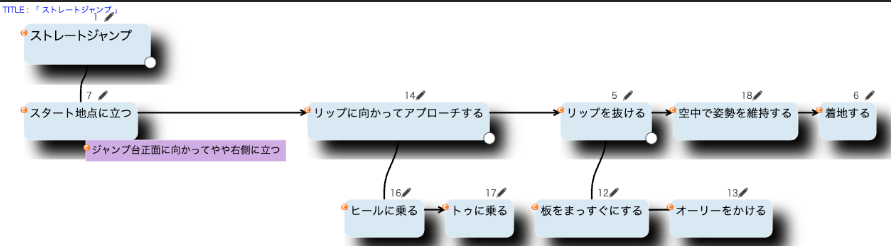
\includegraphics[width=1.0\linewidth]{./image/charm_straight_jump.png}
    \caption{スノーボードのプロセス知識}
    \label{fig6}
\end{figure}

% \begin{figure}[htbp]
%     \centering
%     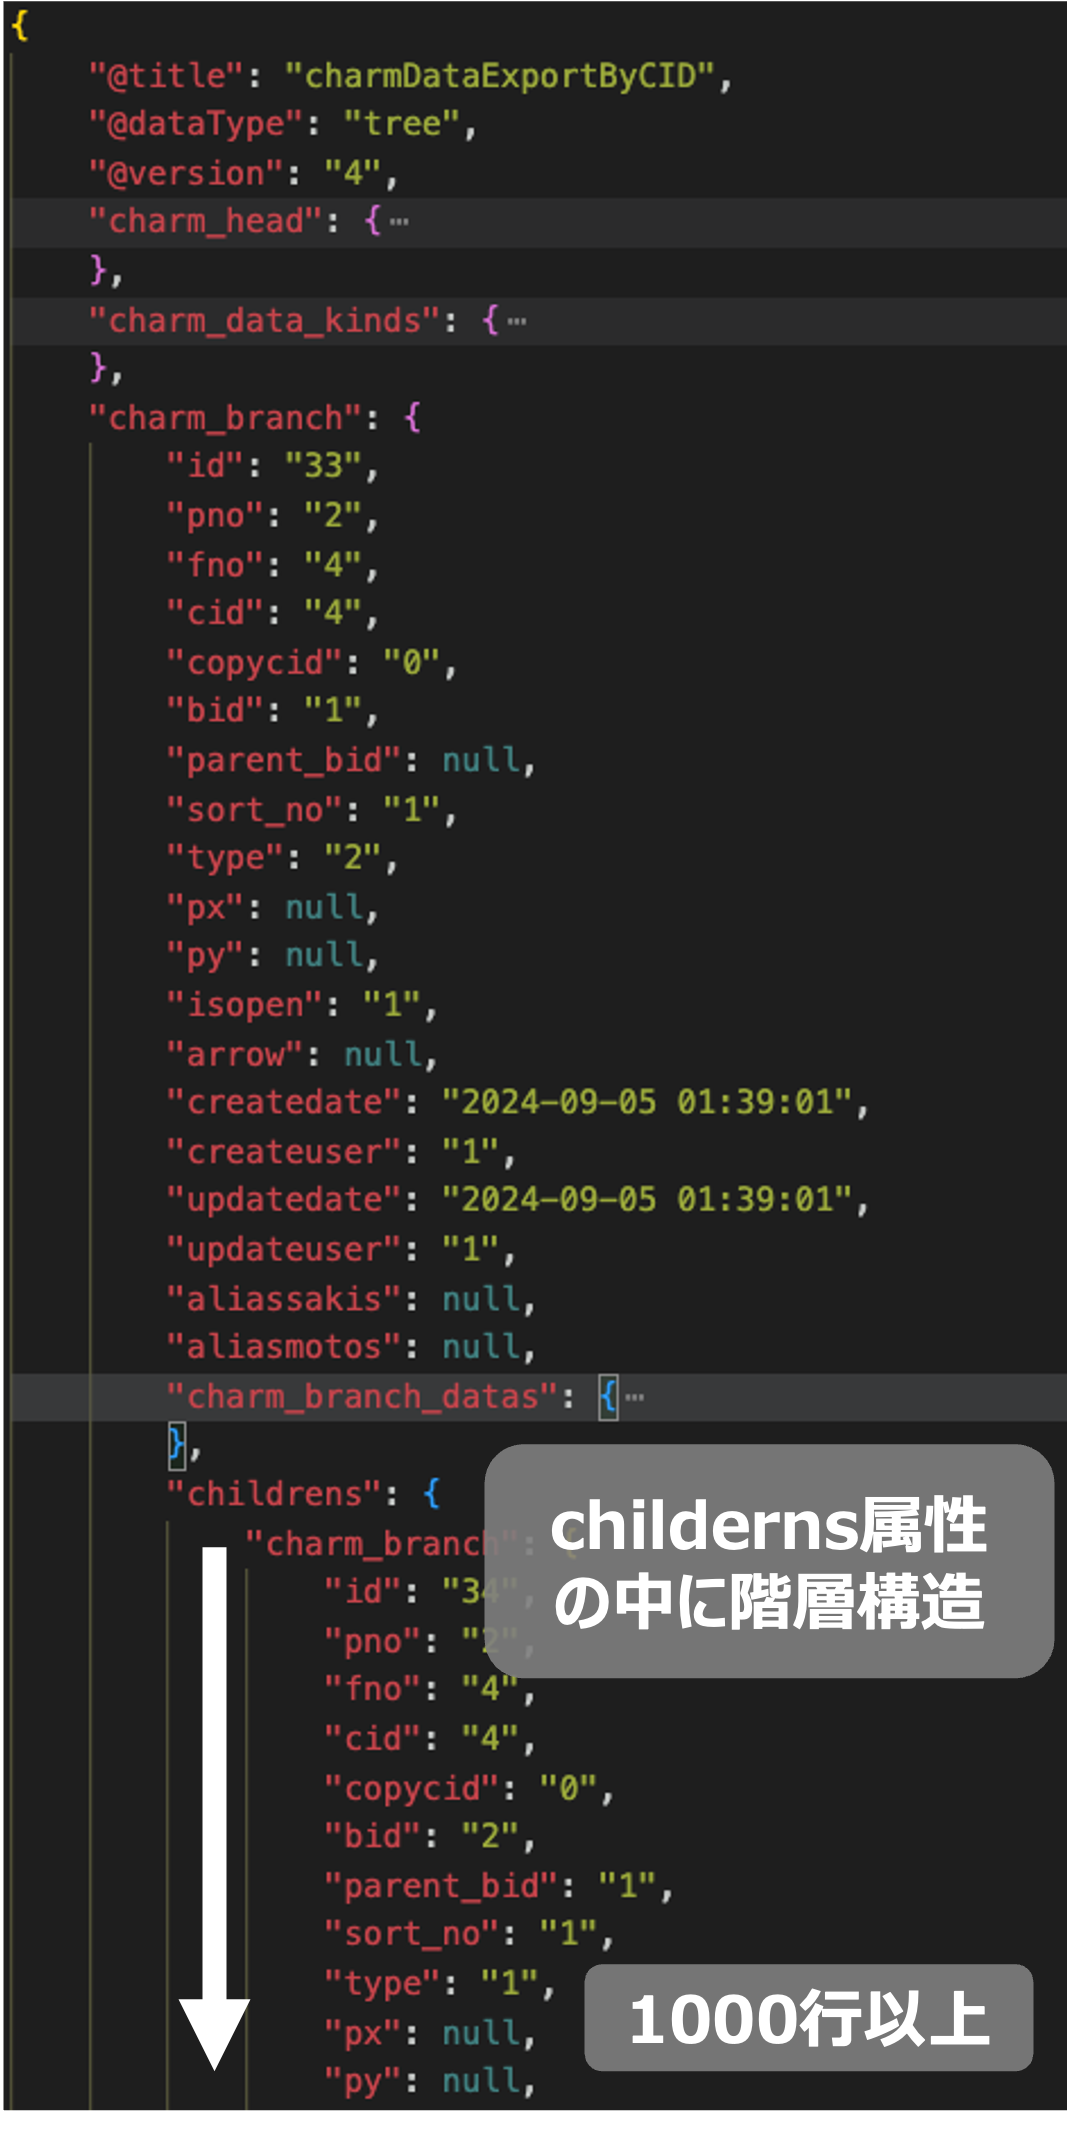
\includegraphics[width=1.0\linewidth]{./image/example_of_json.png}
%     \caption{JSONデータの例}
%     \label{fig_json_example}
% \end{figure}

\subsubsection{実験結果}
社交ダンスのナチュラルターンについて, gpt-4oとClaude Sonnet 3.5の要約結果をそれぞれ図\ref{fig7}と図\ref{fig8}に, スノーボードのストレートジャンプについての要約結果を図\ref{fig9}と図\ref{fig10}に示す.

gpt-4oの要約結果は, 両事例ともJSONに含まれる各属性を淡々と説明するにとどまっている. 一方, Claude Sonnet 3.5は, 対象をそれぞれ「ダンスのステップの手順を詳細に記述したデータ構造」「スノーボードの技に関する手順や知識を構造化して記述したデータ」と特徴づけている. 特筆すべき点として, プロセス知識内には「ナチュラルターン」「ストレートジャンプ」という用語は含まれているものの,「ダンス」「スノーボード」という分野を示す単語は明示されていない. このことから, Claude Sonnet 3.5は専門用語や文脈から対象分野を適切に推論できていることがわかる.

より優れた推論能力を示したClaude Sonnet 3.5に対して, プロセス知識の改良点を問い合わせた結果を図\ref{fig11}, 図\ref{fig12}に示す. 社交ダンスについては, パートナーとの関係性や専門用語(フットアクションの略語等)に関する改良点を指摘している. スノーボードについては, CHARMの並列・順序関係という構造的な観点に加え, 雪質や天候によるジャンプ台の状態といった環境要因についても言及している. これらの結果は, Claude Sonnet 3.5が専門知識とデータ構造の両面から適切な改良提案が可能であることを示している.

以上の検証結果から, 知識抽出支援ツールに使用するLLMのモデルとしてClaude Sonnet 3.5が最適であると判断した.

\begin{figure}[htbp]
    \centering
    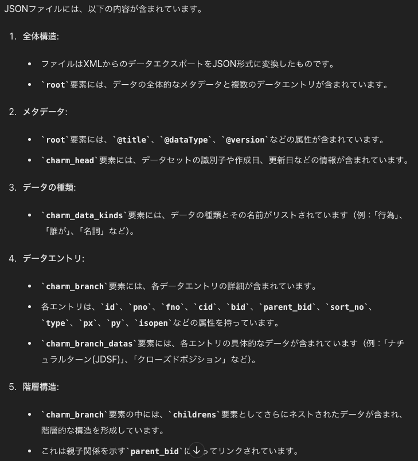
\includegraphics[width=1.0\linewidth]{./image/natural_turn_summarize_gpt4o.png}
    \caption{gpt-4oによる社交ダンスのナチュラルターンに関するプロセス知識の要約結果}
    \label{fig7}
\end{figure}

\begin{figure}[htbp]
    \centering
    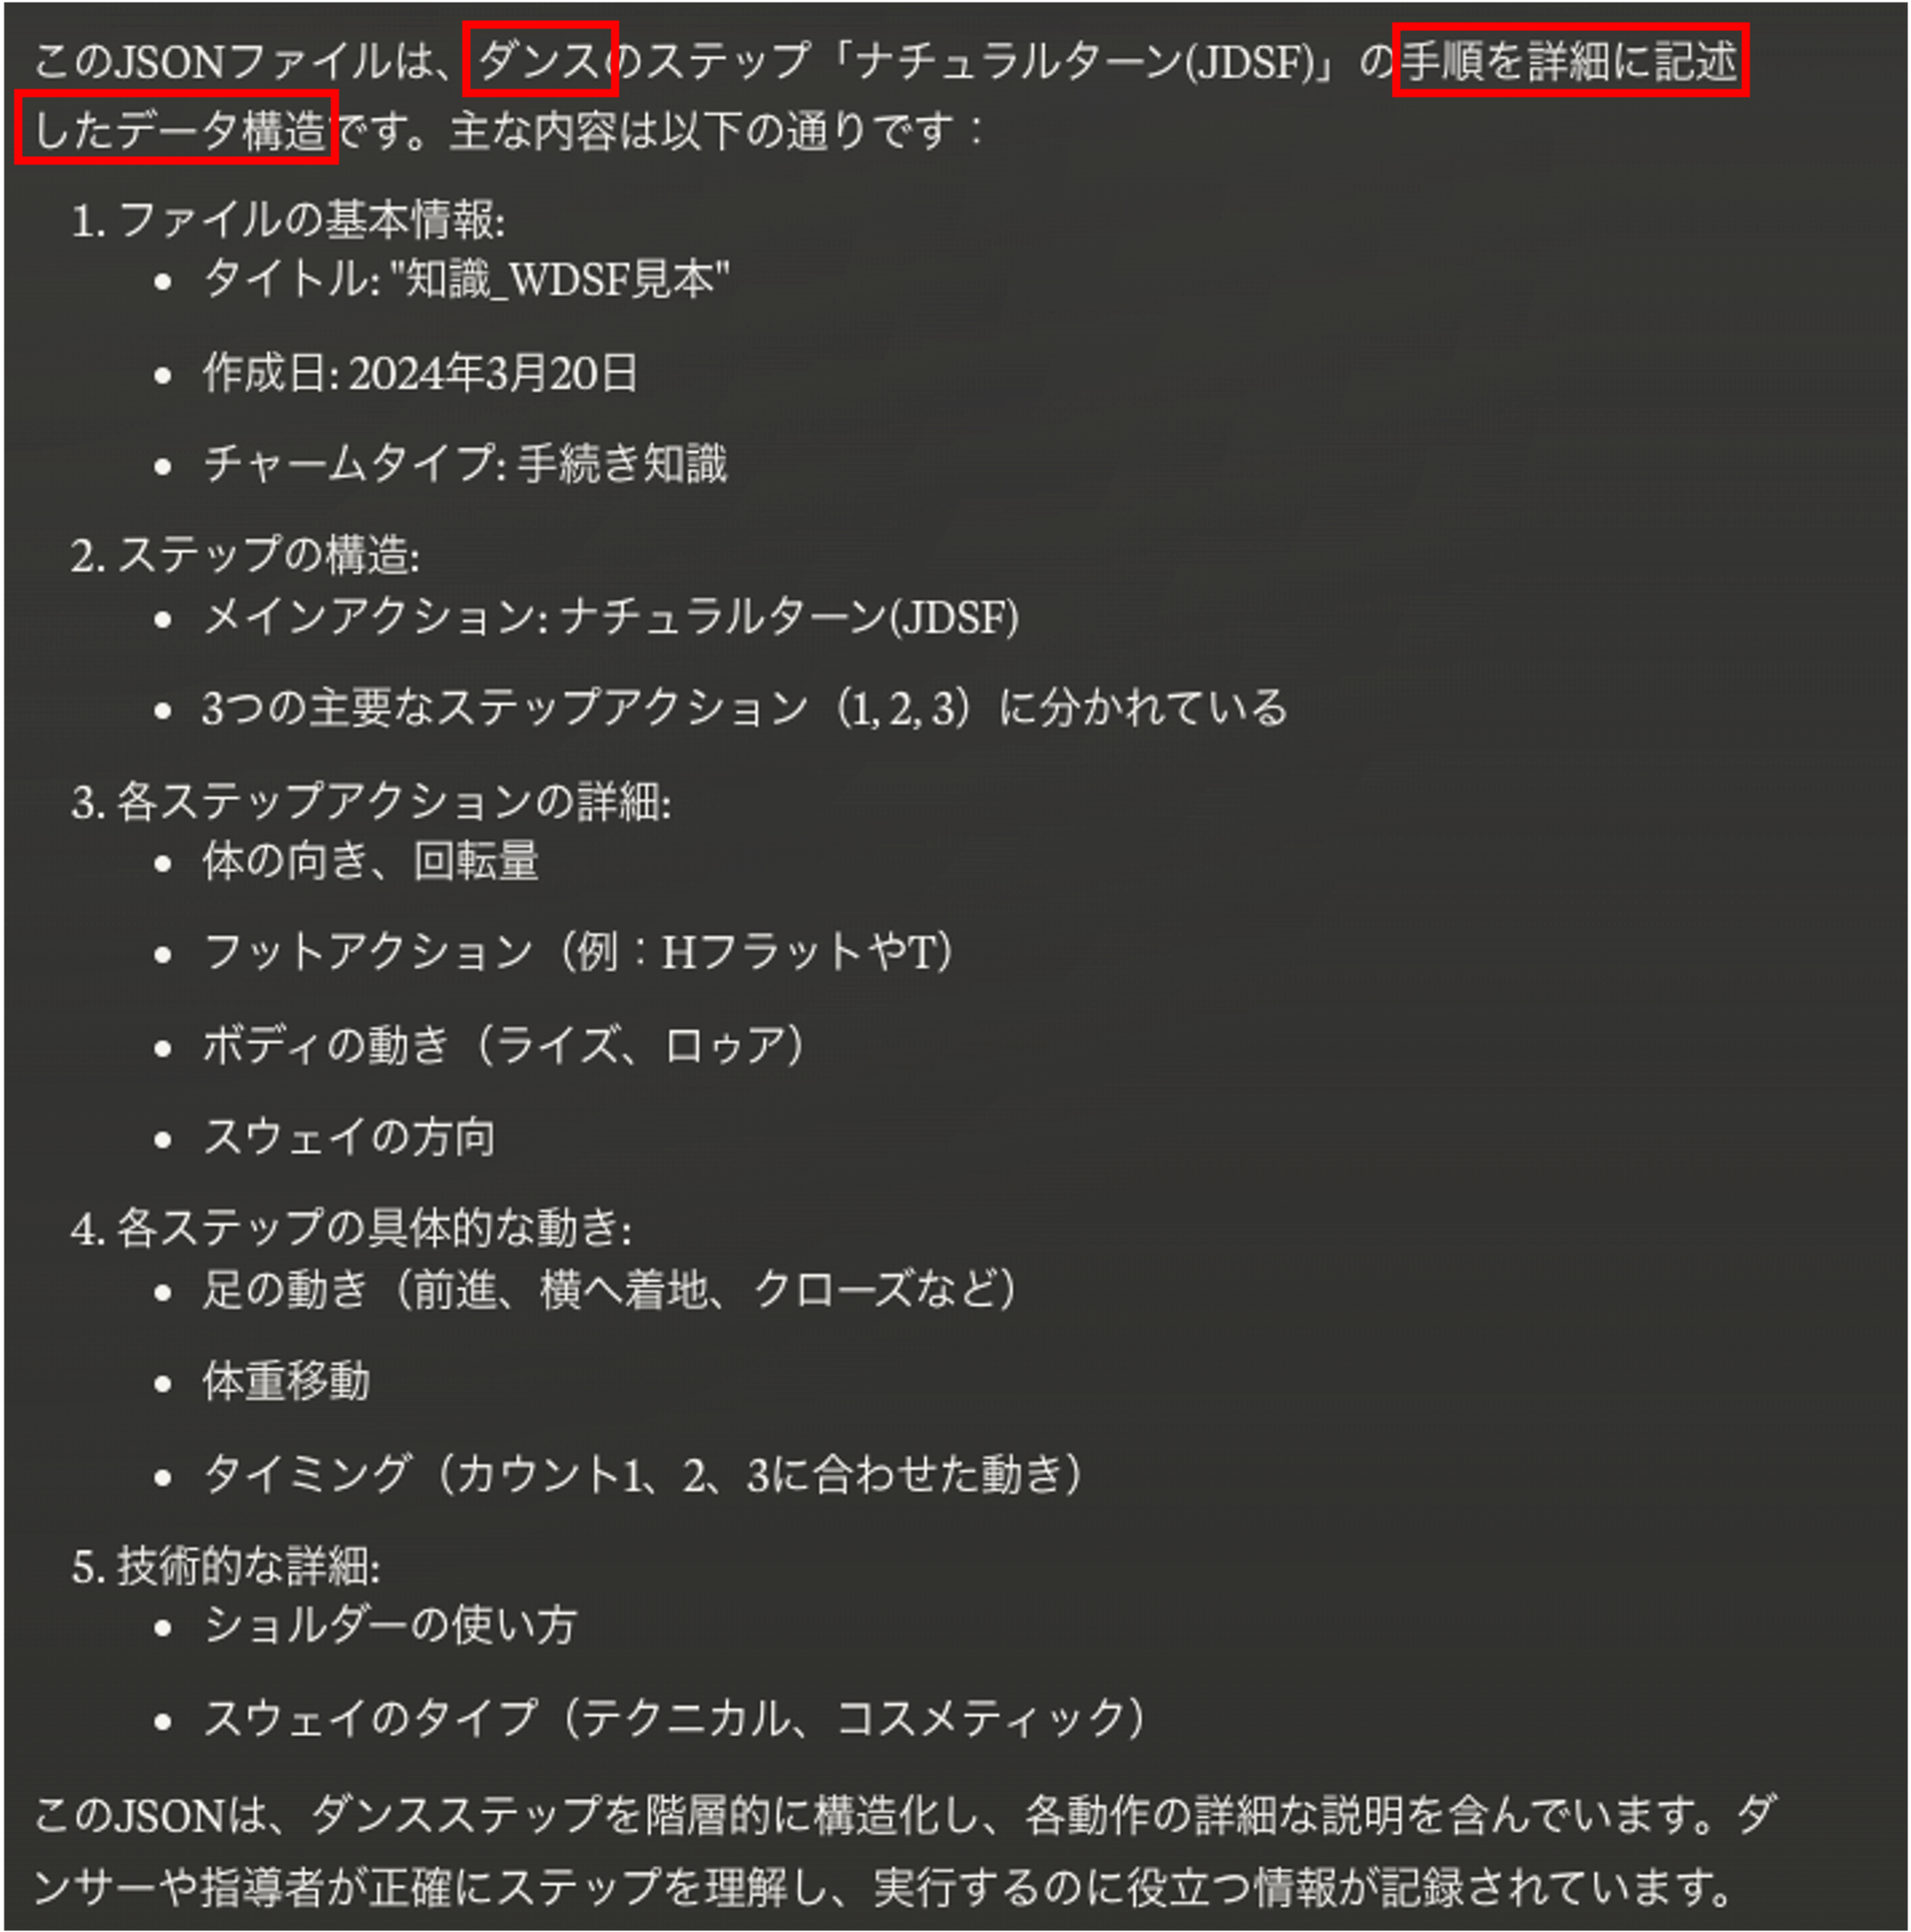
\includegraphics[width=1.0\linewidth]{./image/natural_turn_summarize_sonnet.png}
    \caption{Claude Sonnet 3.5による社交ダンスのナチュラルターンに関するプロセス知識の要約結果}
    \label{fig8}
\end{figure}

\begin{figure}[htbp]
    \centering
    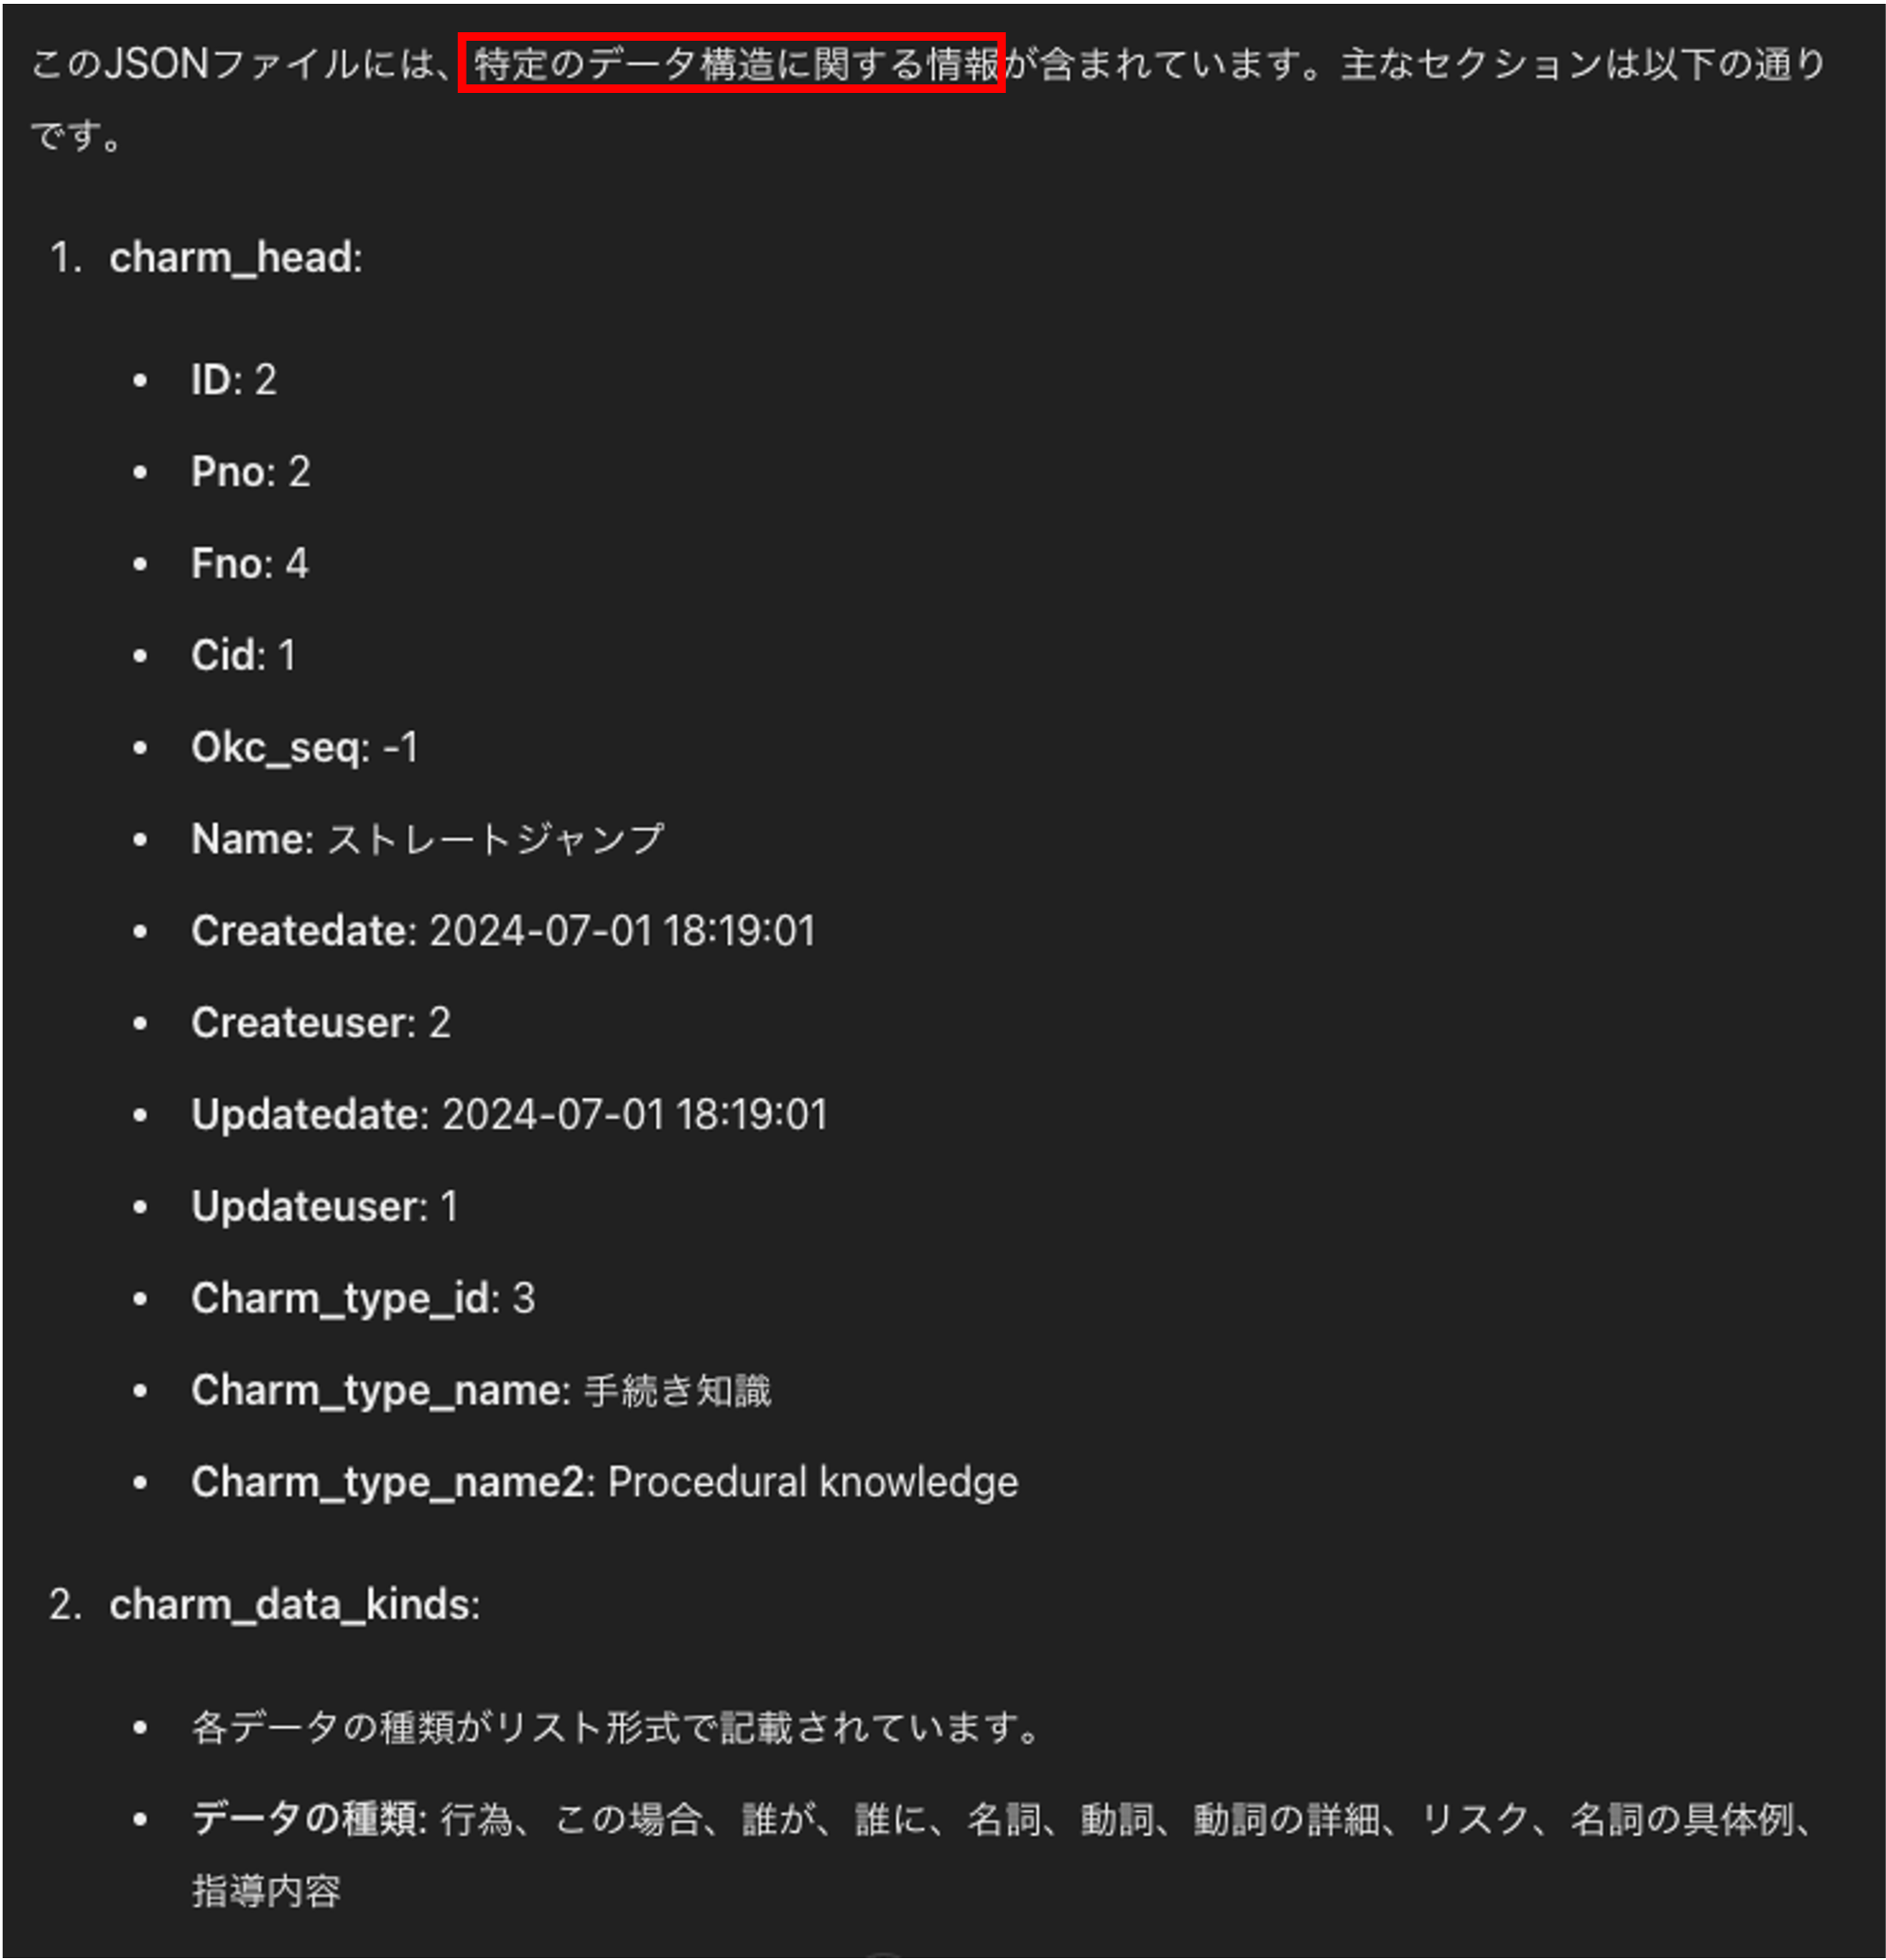
\includegraphics[width=1.0\linewidth]{./image/straight_jump_summarize_gpt4o.png}
    \caption{gpt-4oによるスノーボードのストレートジャンプに関するプロセス知識の要約結果}
    \label{fig9}
\end{figure}

\begin{figure}[htbp]
    \centering
    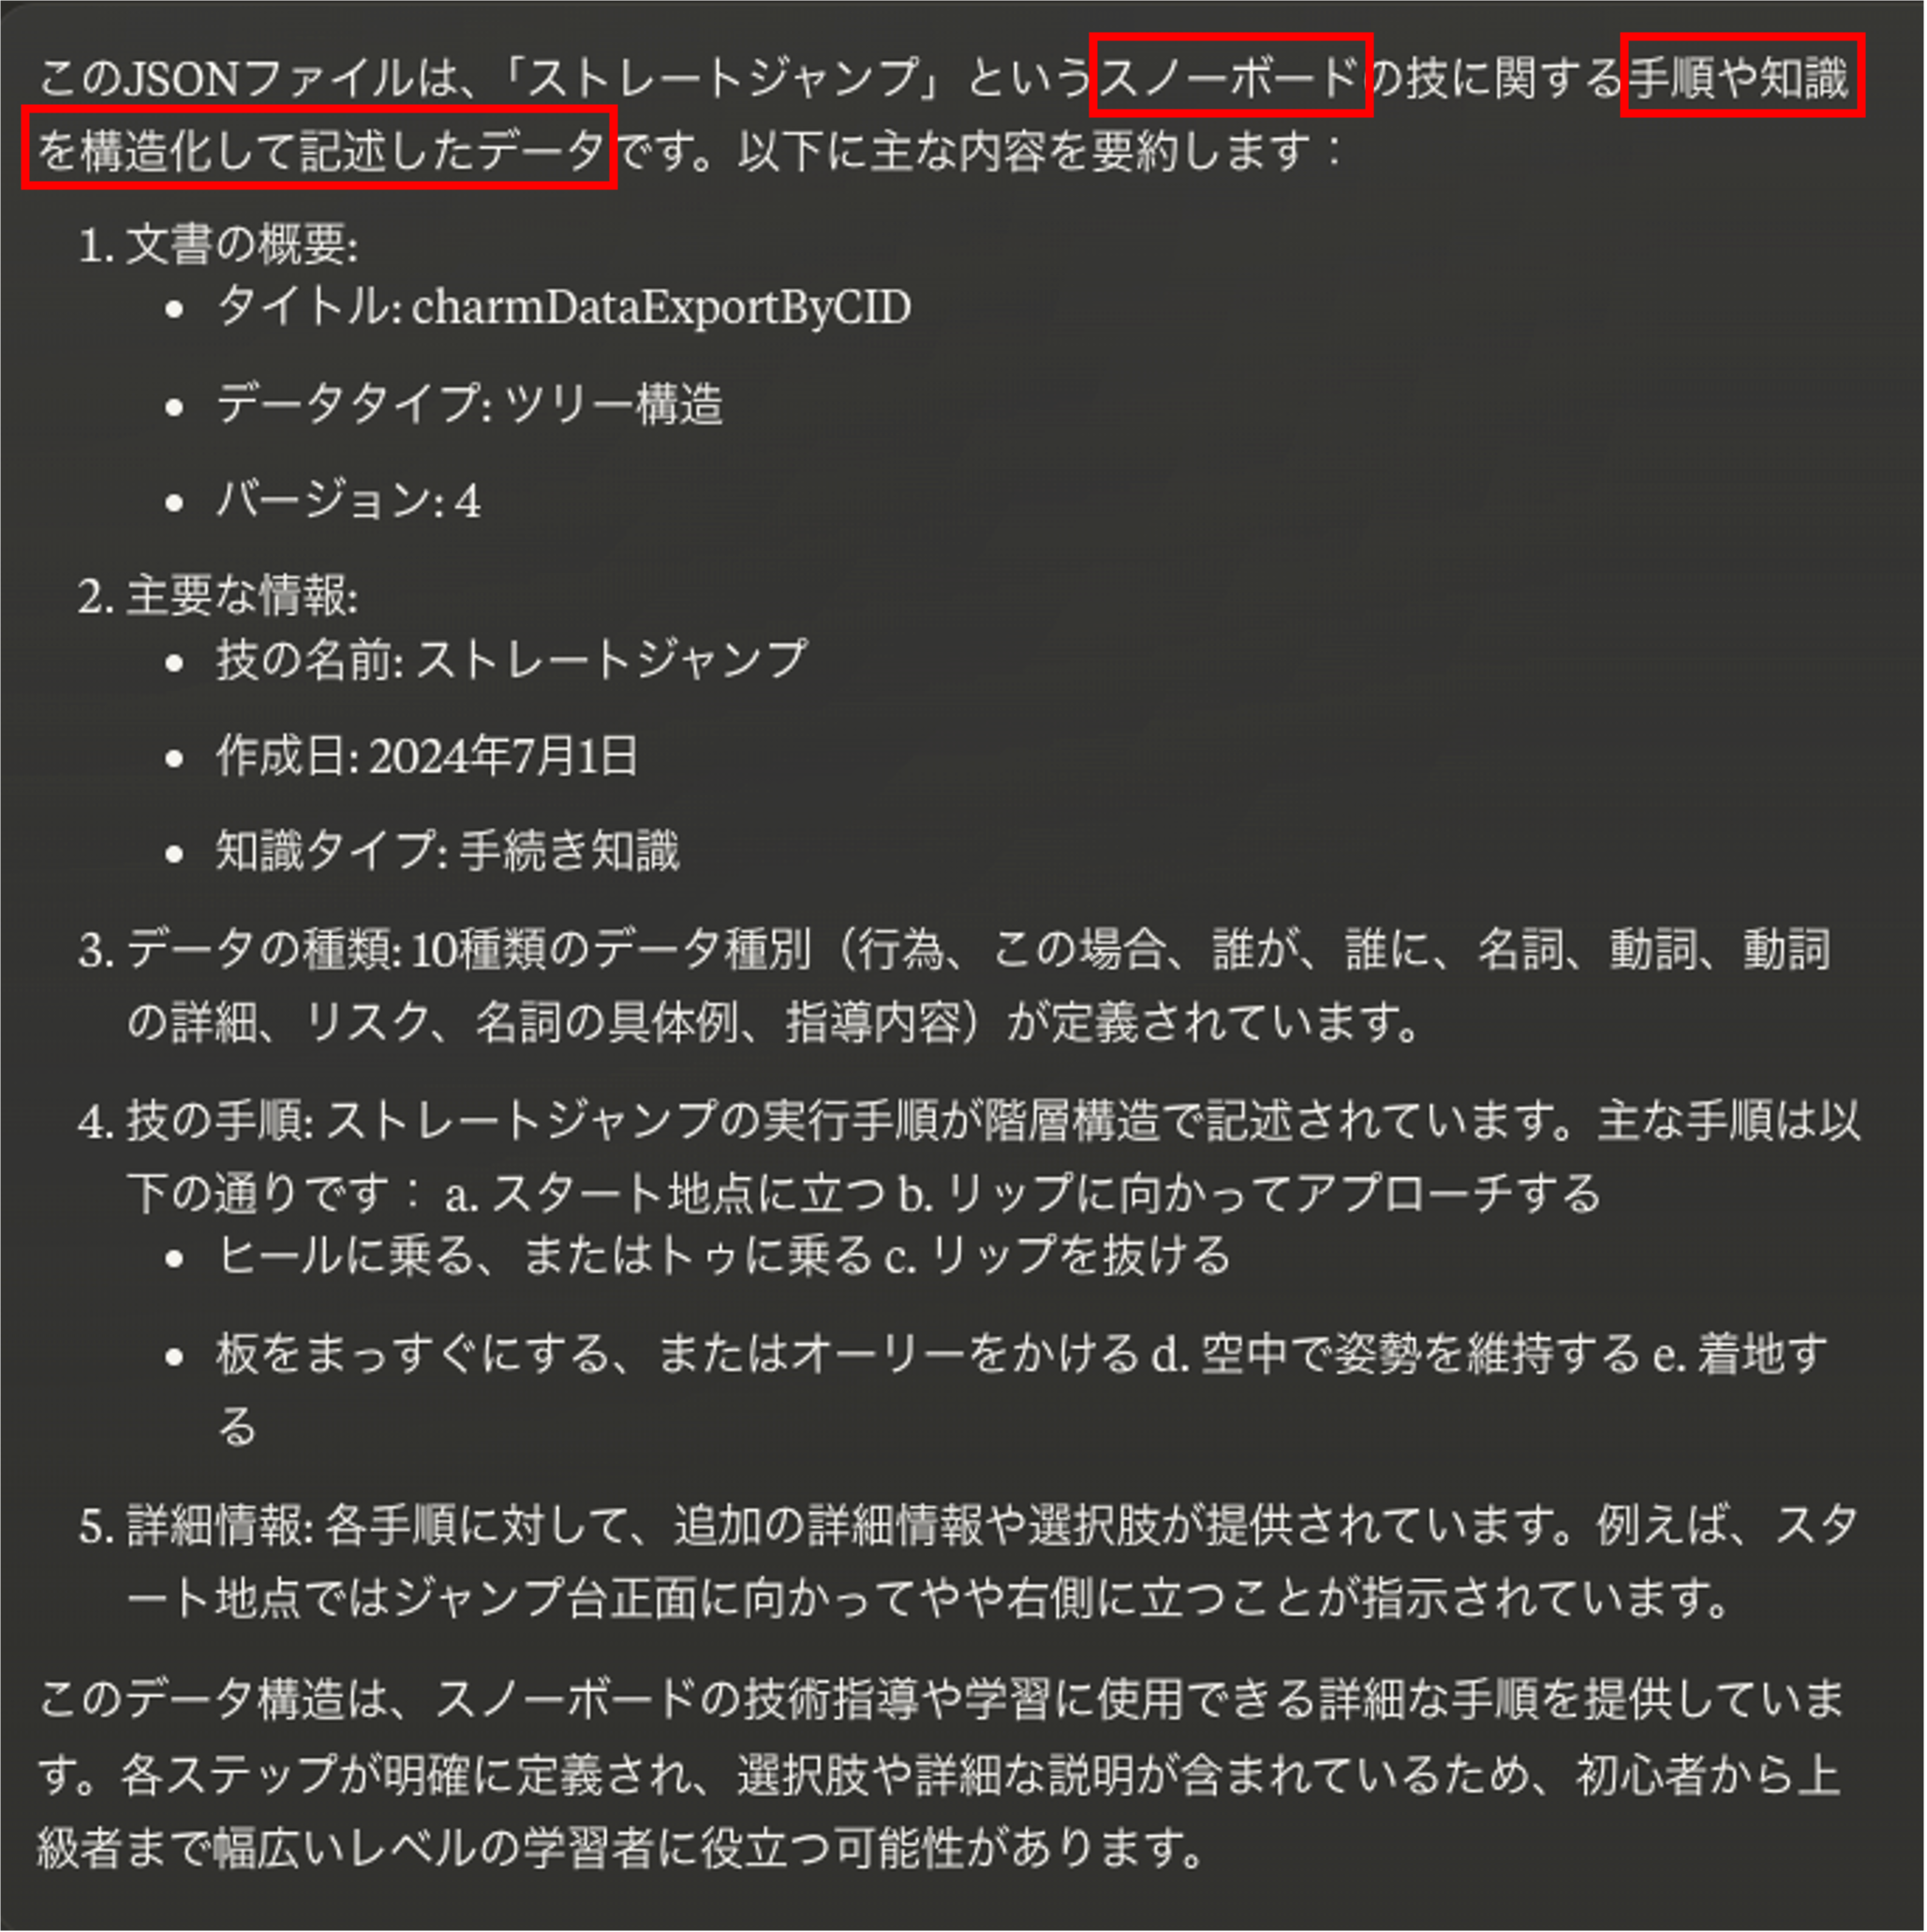
\includegraphics[width=1.0\linewidth]{./image/straight_jump_summarize_sonnet.png}
    \caption{Claude Sonnet 3.5によるスノーボードのストレートジャンプに関するプロセス知識の要約結果}
    \label{fig10}
\end{figure}
\begin{figure}[htbp]
    \centering
    \includegraphics[width=1.0\linewidth]{./image/natural_turn_improvement_sonnet.png}
    \caption{Claude Sonnet 3.5による社交ダンスのナチュラルターンに関するプロセス知識の改良点の提案結果}
    \label{fig11}
\end{figure}

\begin{figure}[htbp]
    \centering
    \includegraphics[width=1.0\linewidth]{./image/straight_jump_improvement_sonnet.png}
    \caption{Claude Sonnet 3.5によるスノーボードのストレートジャンプに関するプロセス知識の改良点の提案結果}
    \label{fig12}
\end{figure}


\subsection{知識抽出における利用可能性の検証}
本項では, 先の実験で利用可能性がgpt-4oより優れていることが示されたClaude Sonnet 3.5について, 知識抽出支援ツールとして最低限の機能を実現できるか検証を行なった.

\subsubsection{実験の設定}
具体的には, 指導者が学習者に指導した内容や学習者とのやり取りの中で, プロセス知識に含まれていない指導コメントと双方向コミュニケーションをLLMが抽出することができるか検証した. 実験協力者は経験年数15年の指導者1人と, 経験年数1年の学習者1人である. プロセス知識としてモデルの選定で使用した社交ダンスのナチュラルターンのプロセス知識(図\ref{fig3})を用いた. 続いて学習者がナチュラルターンを実践している動画を撮影し, 拡張版知識連携アノテーションシステムにアップロードした. LLM評価のために, 指導者に対して,システム上で実指導を行う際に以下の3種類の指導コメントを入力するよう指示した.また指導者は, それらの指導コメントに対して想定される指導者と学習者のやり取りも入力した.

\begin{enumerate}
    \item プロセス知識に記載されていない内容の指導コメントとやり取り
    
    \item プロセス知識に記載されている内容と記載されていない内容の両方を含む指導コメントとやり取り
    
    \item プロセス知識に記載されている内容と一致する指導コメントとやり取り
    
\end{enumerate}

LLMがこれらのコメントのうち, プロセス知識に記載されていない内容を抽出し, その部分についてプロセス知識の改良提案を行うことができるか検証を行なった. 

指導者が付与した具体的な指導コメントを図\ref{fig13, fig14, fig15}に示す. それぞれ先述した1から3の指導コメントの分類に順に対応している.


\begin{tcolorbox}[breakable, colback=white, colframe=black]
    \begin{minted}{text}
-指導コメント- 
    "ダイナミックスウェイをしましょう."

-やりとり- 
    [学習者]:"ダイナミックスウェイとはなんでしょうか?" 
    [指導者]:"骨盤から上を横に傾けることです" 
    \end{minted}
\end{tcolorbox}
    
\captionof{figure}{プロセス知識に記載されていない内容の指導コメントとやり取り} 
\label{fig13}




\begin{tcolorbox}[breakable, colback=white, colframe=black]
    \begin{minted}{text}
-指導コメント-
    “フットアクションはHフラットです. まだ右回転しないようにしましょう.”

-やり取り-
    [学習者]:”ナチュラルターンなので右回転するのかと思いました”
    [指導者]:”右回転は、カウント1の右足を着地し、左足を引き寄せるときに
                発生します. 右足を着地したカウント1では、回転しないように
                しましょう.”

(フットアクションに関する内容はすでにプロセス知識に含まれており, 右回転に
関する記述は含まれていない.)
    \end{minted}
\end{tcolorbox}
    
\captionof{figure}{プロセス知識に記載されている内容と記載されていない内容の両方を含む指導コメントとやり取り} 
\label{fig14}




\begin{tcolorbox}[breakable, colback=white, colframe=black]
    \begin{minted}{text}
-指導コメント-
    “壁斜めに面して進みましょう”

-やり取り-
    [学習者]:”壁斜とは, どちらの方向でしょうか?”
    [指導者]:”ooさんの右斜45度の方向です”
    \end{minted}
\end{tcolorbox}
    
\captionof{figure}{プロセス知識に記載されている内容の指導コメントとやり取り} 
\label{fig15}



また, 作成したプロンプトには以下の内容を記述した。
\begin{enumerate}
    \item 指導現場で発生する情報から熟練技能者の暗黙知を獲得するための方法と順序に関する説明.
    \item プロセス知識に関する基本的な説明.
    \item 指導現場で収集した情報からプロセス知識に含まれていない要素を抽出し, プロセス知識の改良点を提案する旨の指示.
    \item プロンプトチューニング用の詳細な指示文.
    \item 出力の形式.
    \item データ構造の説明.
    \item 入力データの埋め込み.	
\end{enumerate}



\subsubsection{実験結果}
図\ref{fig16}にClaude Sonnet 3.5の出力の一例を示す.

% breakableなtcolorboxで複数ページにわたるコードブロックを表示
\begin{tcolorbox}[breakable, colback=white, colframe=black]
    \begin{minted}{text}
        改良点1:
        <改良の種類>
          改良
        
        <改良位置>
          行為ノードのbid:3
          行為ノードの内容:ステップアクション1を行う
        
        <改良内容>
          {動詞の詳細}属性に以下の内容を追加:
            "カウント1の右足着地時にはまだ回転せず、左
          足を引き寄せる際に右回転を始める"
         
        理由:
          {やりとり情報}の中で、学習者が右回転のタイミ
          ングについて混乱していることが分かります。こ
          の詳細を追加することで、回転のタイミングをよ
          り明確に説明できます。
        
        改良点2:
        <改良の種類>
          追加
        
        <改良位置>
          前行為ノードのbid:9
          前行為ノードの内容:左足を横へ着地する
          後行為ノードのbid:10
          後行為ノードの内容:ボディをリカバーする
        
        <改良内容>
          新しい行為ノードを追加:
            “ダイナミックスウェイを行う”
          理由:
            {指導コメント}と{やりとり情報}でダイナミッ
            クスウェイについて言及されていますが、現在の
            {手順構造化データ}には含まれていません。この
            重要な動作を明示的に追加することで、手順をよ
            り完全なものにできます。
        
        改良点3:
        <改良の種類>
          改良
        
        <改良位置>
            行為ノードのbid:11
            行為ノードの内容:ステップアクション3を行う
        
        <改良内容>
          {動詞の詳細}属性に以下の内容を追加:
            "右足でクローズする際に、左足からの重心移動を
            意識する"
         
          理由:
            現在の説明では、右足に体重を乗せることは言及
            されていますが、左足からの重心移動については
            明確に述べられていません。この詳細を追加する
            ことで、動作の連続性と重心移動の重要性を強調
            できます。
    \end{minted}
\end{tcolorbox}
    
% figure環境は使わず、captionとlabelのみ付与
\captionof{figure}{Claude Sonnet 3.5の出力例} 
\label{fig16}


図\ref{fig16}を見ると, “改良点1”と”改良点2”においてプロセス知識に含まれていない内容の指導コメントに関する言及が見られる. 

“改良点1”ではプロセス知識に記載されている内容と記載されていない内容を含む指導コメントのうち, プロセス知識に記載されていない内容だけを抽出し, 改良点を提案している. 具体的にはやりとり情報から右回転に関する要素を抽出し, ステップアクション1の動詞の詳細プロパティへの追記を促している. 

“改良点2”ではプロセス知識に記載されていない内容を抽出し, 改良点を提案している. 具体的には指導コメントとやりとり情報からダイナミックスウェイに関する要素を抽出し, “左足を横へ着地する”行為ノードと”ボディをリカバーする”行為ノードの間にダイナミックスウェイに関する新たな行為ノードを追加することを促している.

また当出力において, プロセス知識にすでに記載されている”壁斜めに面して進む”ことに関する言及はなかった. 

さらに”改良点3”では指導コメントとやり取りでは一切言及されていない内容に関する改良提案を行っている. これはLLMがプロセス知識を解析し, 独自に行った改良提案である.

次に, この出力結果を指導者に確認してもらった. その時の抜粋及び補足したコメントを図\ref{fig17}に示す.

\begin{tcolorbox}[breakable, colback=white, colframe=black]
    \begin{minted}{text}
-改良点1に対するコメント-
    「(行為ノードを追加する位置は)ある程度位置は合っている.」
    「ダイナミックスウェイは左足を着地した瞬間にやる.(だから, 左足を横へ
     着地する行為ノードの)動詞の詳細にするべき.」
    「(ただし)位置さえわかっていれば(提案の意味を理解して修正する位置を)
     人間が調整できる.」

-改良点2に対するコメント-
    「(この提案は)やりとりを要約しただけ.」
    「内容は合っている.」

-改良点3に対するコメント-
    「(提案の内容は, 指導者の)コメントとしてあり得る.」
    「実際に(重心移動を)できない人もいるので(この提案は)重要.」
    \end{minted}
\end{tcolorbox}
    
\captionof{figure}{指導者のLLMの出力に対するコメント} 
\label{fig17}


図\ref{fig17}から, LLMの出力は指導者から見ても改良位置や内容についておおよそ合っていると考えられる. また, 改良点1に対する指導者のコメントから, LLMの改良提案に誤差があっても人間の確認によって補完できる範囲内であることが伺える. さらに, 改良点3に対する指導者のコメントから, LLMが指導者も重要だと考えるプロセス知識の改良提案をできていることがわかる. 

\subsection{インターフェイスの実装}





% 第5章{結果}
\chapter{提案手法の有効性検証}

\section{検証の目的}
 提案手法の有効性を検証するための実験を行った. 本研究は, 知識発現\cite{Nishimura2017}における課題に対して, 指導現場での対話収集とLLMの活用という複合的なアプローチによる解決を提案している. 具体的には, 以下の2点を主な評価項目とした.\\
\begin{enumerate}
    \item 指導現場での知識抽出の有効性:\\
    指導現場おいて, 指導者の発話内容や学習者との対話から, プロセス知識に含まれていない新たな知見が得られるかを検証する. 
    \item LLMによる知識抽出支援の有効性:\\
    収集された指導事例からLLMが提案する改良点が, 実際の指導内容を適切に反映しているか, また体系的な知識整理に寄与しているかを検証する. これは, 記述漏れの検出や知識の体系化という課題に対するLLMの有効性を示すものである. 
\end{enumerate}


\section{実験方法}
\subsection{実験環境}
 本実験は, 石川県内のダンススタジオの協力を得て実施した. 実験協力者として指導者2名と学習者13名が参加した. 指導者の経験年数は, 指導者Aが35年, 指導者Bが30年であった. また, 学習の中で経験年数を回答した8名のうち5名が経験年数1年, 2名が2年, 1名が3年であった.なお, 本実験は本学(北陸先端科学技術大学院大学)の知識科学倫理審査会議の承認(承認コードKSEC 人04-038)に基づいており, 実験協力者に対しては実験の目的, データの収集・利用方法, 個人情報の保護, 参加の任意性等について説明を行い, 同意を得た. \\
 実験対象として社交ダンスのクカラチャを選定した. 社交ダンスを選定した理由は, これまで知識発現が対象としてきた製造業や介護現場とは異なる特徴を持つと考えられるためである. 製造業や介護の現場では, 作業手順や判断基準といった知識を, 実務経験から想起して言語化することが求められる. これに対して社交ダンスでは, 動作の正確さを客観的な基準で判断することが本質的に困難であると考えられる. 例えば「美しい」アームワークや「良い」ステップといった評価は, 指導者の主観的な理解に基づいている. そのため指導者は, 自身が持つ評価基準や動作の意図を, その場で学習者が理解できる形に言語化して伝える必要がある. このとき, 「腕の高さをここまで上げる」「体重移動のタイミングをここで行う」といった具体的な指示から, 「なぜその動きが必要か」「どのような効果を意図しているか」といった原理的な説明まで, 様々な知識が自然と言語される可能性がある. \\
 さらに, この言語化は学習者の実践に基づいて行われる. 例えば製造業では, 作業の結果が製品の品質として客観的に評価できるため, 指導者は事前に想定される状況に対する判断基準を説明することができる. 一方, 社交ダンスでは学習者が実際に動作を行う中で「なぜこの動きがうまくいかないのか」「どうすれば改善できるのか」といった具体的な疑問が生まれ, それに応える形で指導者の持つ知識が表出されると考えられる. これは, ワークショップのように意図的に知識を想起する場合とは異なり, 実践の文脈に即した形で必要な知識が引き出されることを意味する. \\
 また, 社交ダンスの中でもクカラチャを選定した理由は, クカラチャはルンバの基本となるステップであり, 社交ダンスにおいて特に重要な技術だからである. \\
 こうした理由から, 提案手法の有効性検証の題材として社交ダンスのクカラチャを選定した.\\
\\


\subsection{実験手順}
\subsubsection{プロセス知識の構築}
 初めに, 知識発現手法に基づき, クカラチャのプロセス知識を構築した. まず社交ダンスの教科書を基に初期のプロセス知識を作成した. その後, オンライン会議システム(Zoom)を用いて指導者へのヒアリングを実施し, 内容の確認と改良を行った. これを本検証のベースとなるプロセス知識とした.\\


\subsubsection{データ収集の基本手順}
 実験期間は2023年10月16日から11月13日までの約5週間とした. 動作の撮影にはスマートフォンのカメラを使用し, システムへのアクセスについては指導者はPCを, 学習者は各自のスマートフォンを使用した. なお, 学習者の参加回数は個人によって1回から3回まで幅があった. また, クカラチャの実践時に使用した音楽は「Maroon5 Memories」であった.\\
 実験開始時に, 指導者と学習者に対して各種システムの使用方法を説明し, 実際の操作を体験する機会を設けた. 具体的には, アノテーションシステムへのログイン方法, 動画の視聴方法, コメントの確認方法, およびチャット機能の使用方法について説明を行った.\\
 週1回のレッスン日における基本的なデータ収集の手順は以下の通りである.\\
\begin{enumerate}
    \item 指導者がクカラチャの基本動作について説明と実演を行い, 学習者が練習を行った
    \item 研究者が学習者の動作をスマートフォンで撮影し, システムにアップロードした. 撮影の際は, 学習者の全身が画角に収まるよう配慮した
    \item レッスン後, 指導者がPCを使用して動画に指導コメントを付与した
    \item 次のレッスンまでの1週間の間に, 学習者は付与された指導コメントを確認し, 必要に応じて質問や感想を投稿した. また指導者は質問があれば適宜応答した
\end{enumerate}

\subsubsection{プロセス知識の更新プロセス}
 実験開始時に, 指導者には実験期間中にプロセス知識の改良が必要だと感じた場合は随時更新可能である旨を説明した. これは, 指導現場での気づきやLLMによる改良提案を受けて, プロセス知識をより適切なものに改善していくことを意図したものである. プロセス知識の更新は, (1)実験期間中の指導者からの自発的な更新, (2)実験終了後のLLMの妥当性評価を受けての更新, という2つの機会を設けた.\\

\subsubsection{実験中の改善施策}
 実験の進行に伴い, 以下の改善を実施した.\\

\begin{enumerate}
    \item 指導者の見本動画の追加:\\
    より正確な動作イメージを学習者に共有するために, 指導者の見本動画もシステムにアップロードした.
    \item システム利用状況の把握とフォローアップ:\\
    研究者が定期的にシステムの利用状況を確認し, 必要に応じて操作方法の再説明等のフォローアップを実施した. また, LINEを用いて定期的にシステム利用の促進を行った.
    \item システム利用状況の問題切り分け:\\
    システム利用率の低さの原因を特定するため, 学習者には指導コメントを確認した際に必ず「ありがとうございます」などの返信を行うよう指示した. これにより, コメントを確認していない場合と, 確認したが返信していない場合を区別することが可能となった.
\end{enumerate}


\subsection{評価方法}
 実験期間終了後, 提案手法の有効性を検証するため, 以下の4つの観点から評価を実施した. \\
\begin{enumerate}
    \item 指導現場における新しい知識の抽出可能性
    \item LLMが出力した改良提案の適切性
    \item プロセス知識の改良結果
    \item 学習者による提案手法の受容性
\end{enumerate}
 それぞれの評価の目的と具体的な評価方法は以下の通りである.

\subsubsection{指導現場における新しい知識の抽出可能性の評価}
 本評価の目的は, 指導現場が知識抽出の場として有効に機能するかを検証することである. この評価目的に対し, 収集した指導事例について, 定量的評価と定性的評価を実施した. 定量的評価では, 指導コメント数ややり取り数などの基本統計, およびプロセス知識に含まれない要素(未含有要素)の割合を分析した. 定性的評価では, 指導コメントの内容分類とやり取りの特徴分析を行った.\\
 なお, 未含有要素の判定は研究者(社交ダンス未経験者)が行った. 以下のいずれかに該当する指導コメントを「未含有要素を含む」と判定した.\\
\begin{itemize}
    \item 構造化知識を参照しても理解できない要素を含むコメント
    \item コメントの意図は理解できるが, その内容が構造化知識に明示的に含まれていないコメント
\end{itemize}

\subsubsection{LLMが出力した改良提案の適切性評価}
 本評価の目的は, LLMが知識抽出支援ツールとして有効に機能するかを検証することである. この目的に対し, 定量的評価と定性的評価を実施した. 定量的評価では, 以下の3つの観点から評価を行った.\\
\begin{enumerate}
\item LLMが指導現場から得られた指導コメントとやりとりから未含有要素を抽出できているか
\item LLMが指導現場から得られた指導コメントとやりとりからプロセス知識に既に含まれる要素を除外できているか
\item 改良提案の内容および提案位置が適切かどうか
\end{enumerate}
 このうち, 1と2については先述した研究者による未含有要素, 既存要素の分類を正解データとして, Accuracy, Precision, Recall, F値を評価指標を用いた. 3については出力をしづオシャに評価してもらい, Accuracyを算出した.
また, LLMの出力を得る際は, 入力として全ての指導コメントとやりとりを一度にプロセス知識に紐づけることも技術的には可能だが, 改良提案の適切性をより厳密に評価するため, 本実験では個別に紐づけて評価を行った. \\

\subsubsection{プロセス知識の改良結果の評価}
 本評価の目的は, 提案手法が熟練技能者の持つ知識を自然に抽出・整理可能な仕組みとして機能するかを検証することである. この目的に対し, 以下の2つの機会におけるプロセス知識の改良内容を確認した.\\
\begin{enumerate}
\item 実験期間中の自発的な改良:指導者には実験期間中, 気づきがあれば随時プロセス知識を更新可能である旨を伝え, その結果としての改良内容
\item LLMの改良提案を受けての改良:実験終了後, LLMが出力した改良提案の適切性評価を踏まえて実施された改良内容
\end{enumerate}

\subsubsection{学習者による提案手法の受容性評価}
 本評価の目的は, 提案手法が自然な文脈での知識抽出・整理の仕組みとして成立するために必要な, 学習者からの支持が得られているかを検証することである. 指導現場における知識抽出・整理は, 学習者がその仕組みを受け入れ, 積極的に活用することで初めて実現されるためである. この検証のため, 学習者へのアンケート調査(13名中8名が回答)およびシステムの使用感や改善点に関するヒアリングを実施した. アンケートでは以下の項目について調査を行った:\\
\begin{enumerate}
\item 学習者の基本情報
    \begin{itemize}
        \item 社交ダンスを始めた目的
        \item 経験年数
        \item 普段の練習時間・場所
    \end{itemize}
\item 普段の学習方法
    \begin{itemize}
        \item 指導内容の理解・記憶方法
    \end{itemize}
\item システムの利用状況
    \begin{itemize}
        \item システムの確認頻度
        \item システムの利用方法
        \item クカラチャへの理解深化要因
    \end{itemize}
\item 自由記述
    \begin{itemize}
        \item システムの使用感
        \item 本研究への要望
        \item その他感想
    \end{itemize}
\end{enumerate}


\section{評価結果}
 ここでは, 収集したデータに基づいて提案手法の有効性に関する評価結果を示す. まず事前に準備したプロセス知識の概要を説明する. 続いて各評価項目について, 定量的な評価と定性的な評価の結果を示し, これらを踏まえて提案手法の有効性を考察する.




\subsection{事前準備したプロセス知識の概要}
 実験に先立ち, クカラチャの動作を構造化したプロセス知識を作成した. 図\ref{fig:process_knowledge_base}は, その一部であるレフトフットクカラチャ(男子)の動作を示したものである. なお, ライトフットや女子の動作については, 基本的な構造は同じで動作の向きが逆になるのみである.\\

\begin{figure}[htbp]
    \centering
    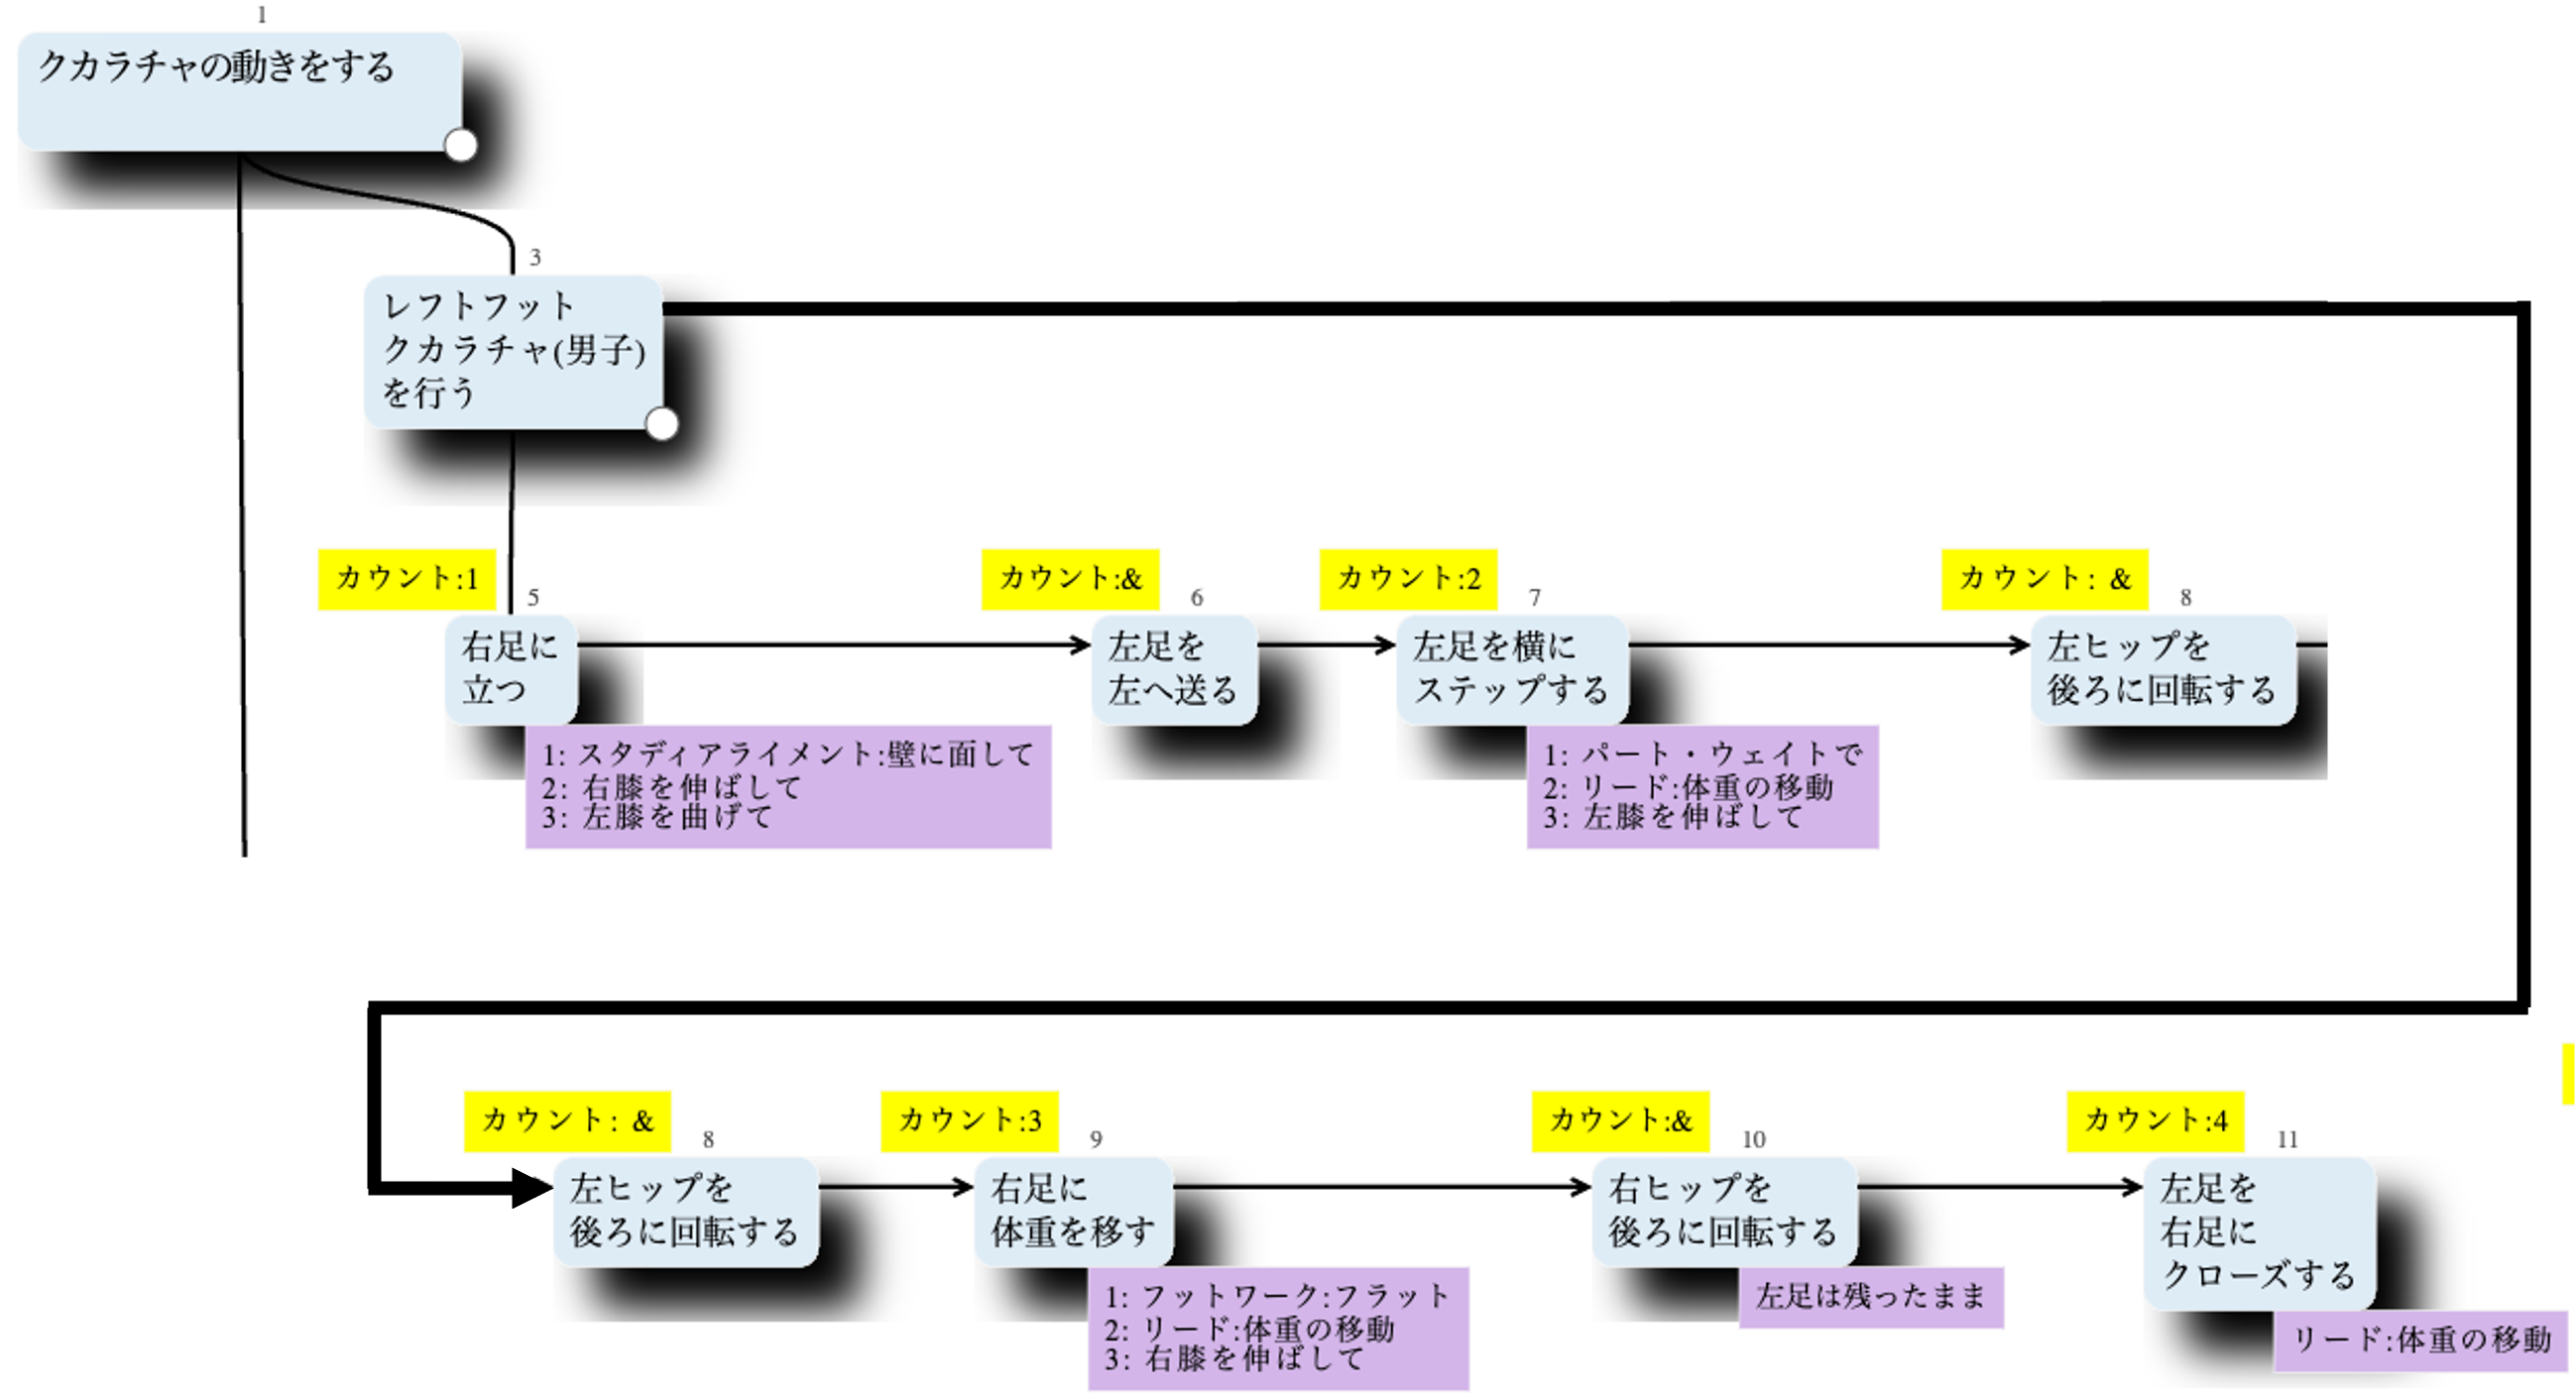
\includegraphics[width=1.0\linewidth]{./image/process_knowledge_base.png}
    \caption{レフトフットクカラチャ(男子)のプロセス知識}
    \label{fig:process_knowledge_base}
\end{figure}

 このプロセス知識は, 7つの基本動作(右足に立つ, 左足を左へ送る, 左足を横にステップする, 左ヒップを後ろに回転する, 右足に体重を移す, 右ヒップを後ろに回転する, 左足を右足にクローズする)で構成されている. それぞれの動作には実行タイミング(カウント)が設定されており, また「スタディアライメント:壁に面して」「パート・ウェイトで」「フットワーク:フラット」といった動作の詳細な指示が付与されている.\\



\subsection{指導現場における新しい知識の抽出可能性の評価}
\subsubsection{定量的評価}
 収集した指導コメントについて, プロセス知識に含まれている要素のみで構成されるもの(以下, 既存要素のみ)と, プロセス知識に含まれていない要素を含むもの(以下, 未含有要素を含む)に分類して分析を行った.\\
 プロセス知識との対応関係について, 既存要素のみで構成されるものが12件(約24\%), 未含有要素を含むものが37件(約76\%)であった. この37件の未含有要素を含むコメントのうち, 指導者1のコメントが12件, 指導者2のコメントが25件を占めていた.\\
 やり取りの特徴として, 全49件の指導コメントのうち18件(約37\%)に学習者とのやり取りが存在した. やり取りの回数については, 1回のやり取りで終了したものが16件, 3回のやり取りに及んだものが2件であり, 1つの指導コメントに対する平均やり取り数は1.22回であった.\\

\subsubsection{定性的評価}
 収集された指導コメントには, プロセス知識を詳細化する指導と, プロセス知識に記載のない新しい部位に関する指導が見られた.\\
 プロセス知識を詳細化する指導では, 「踏み替えのタイミングが早い」「左足に体重が乗る前にヒップが回転してしまっている」といった動作の順序やタイミングに関する指摘や, 「軸が左足内側まで乗るように」「踏みかえの体重移動をはっきりと」といった体重移動の詳細な方法に関する指導が含まれていた. また,「ヒップと一緒にももも外側に回転させる」「左のヒップを回転した時に左の内ももを後ろにひく」といった既存の動作要素をより詳細に説明する指導や, 「ボディの移動は早く, ヒップのアクションはゆっくり見せるとメリハリがでる」といった動作の質に関する指導も見られた.\\
 プロセス知識に記載のない新しい部位に関する指導としては, 「ボディをストレッチ」「上半身, アームの動きがぎこちない」「上半身が揺れて傾いてしまう」といった上半身の使い方に関する指導が見られた. これらはプロセス知識では言及されていなかった身体部位の動きについて説明するものであった.\\
 やり取りについては, 全22件中16件が「ありがとうございます」といった単純な確認や感謝のコメントであった. 一方で, 残りの6件では指導内容に関する具体的なやり取りが見られた. 例えば, 「体重移動しながら回転させてしまってる」という学習者の質問に対し, 指導者が「歩幅を少し狭めた方が体重移動とヒップの回転を分けられる」と回答するなど, 対話を通じてプロセス知識には含まれていない動作の詳細が明らかになる場面も観察された.\\

\subsubsection{知識抽出の場としての有効性}
 定量的な評価と定性的な評価の結果から, 指導現場が知識抽出の場として効果的に機能することが確認された. まず, 収集された指導コメントの76\%(37件)に未含有要素が含まれていたことは, 指導現場が新たな知識を抽出する機会を多く含んでいることを示している.\\
 定性的評価で示したように, 指導現場では2つの方向で知識が抽出されていた. 1つ目はプロセス知識の詳細化である. 体重移動の詳細な方法や動作の質的な側面など, プロセス知識では表現しきれていなかった要素が具体的な指導を通じて明らかになった. 特に動作の順序やタイミングに関する指摘は, プロセス知識で示された基本的な動作の関係性をより正確に理解する上で重要な知見となった.\\
 2つ目は上半身の使い方など, プロセス知識では言及されていなかった新しい部位に関する指導である. これらの指摘は, クカラチャの動作がプロセス知識に記述された下半身の動きだけでなく, 全身の協調的な動きとして捉える必要があることを示している.\\
 さらに, 37\%の指導コメントで学習者とのやり取りが確認された. その中でも特に注目すべきは, 学習者からの具体的な質問に対する指導者の回答を通じて新たな知識が表出される場面である. 定性的評価で示した体重移動と回転の分離に関するやり取りは, 学習者の問題提起が新たな指導内容を引き出すきっかけとなることを示す例である.\\
 このように, 指導現場では, プロセス知識の詳細化や新たな知識要素の発見が自然な形で行われることが確認された. 特に学習者との対話は, プロセス知識には含まれていない要素を引き出す重要な機会となっていた.\\
 一方で, やり取りの発生は全指導コメントの37\%にとどまり, そのうち73\%(16件)は「ありがとうございます」といった確認や感謝のコメントであった. このことは, 指導現場での双方向のコミュニケーションを十分に引き出せていない可能性を示している. この要因については, 後述する学習者へのアンケート結果から示唆が得られている.\\
 これらの結果は, 指導現場が知識抽出の場として大きな可能性を持つことを示している. 特に, プロセス知識の詳細化と新たな知識要素の発見という2つの方向性での知識抽出が確認されたことは, 提案手法の有効性を支持するものである. しかしながら, 双方向コミュニケーションの活性化という点では課題が残されており, より効果的な知識抽出を実現するためには, 学習者の積極的な参加を促す仕組みの改善が必要であることも明らかになった. 


\subsection{LLMが出力した改良提案の適切性評価}
\subsubsection{定量的評価}
 LLMが分析した改良点と提案内容について, 未含有要素の抽出と既存要素の除外, および改良提案の適切性という3つの観点から評価を行った.\\
 まず, プロセス知識との対応関係に着目した評価結果を表\ref{table_llm_extraction}に示す.

\begin{table}[htbp]
    \centering
    \begin{tabular}{l|rrrr}
        \hline
        評価項目 & Accuracy & Precision & Recall & F値 \\ \hline
        未含有要素の抽出 & 0.865 & 0.941 & 0.914 & 0.928 \\
        既存要素の除外 & 0.583 & 0.500 & 0.200 & 0.286\\
        \hline
    \end{tabular}
    \caption{LLMによる要素の抽出・除外の評価結果}
    \label{table_llm_extraction}
\end{table}

次に, LLMによる改良提案の評価結果を表\ref{table_llm_proposal}に示す. ここでは, 指導現場で収集した指導コメントやそのやり取りから直接的に導かれる「指導事例に基づく提案」と, LLMが持つ知識に基づいて補完的に生成する「指導事例に基づかない提案」に分けて評価を行った.

\begin{table}[htbp]
    \centering
    \begin{tabular}{l|l|rrrr}
        \hline
        提案の種類 & 評価観点 & Accuracy \\ \hline
        \multirow{2}{*}{指導事例に基づく提案} & 内容 & 0.780 \\
        & 位置 & 0.361 \\ \hline
        \multirow{2}{*}{指導事例に基づかない提案} & 内容 & 0.254 \\
        & 位置 & 0.182 \\
        \hline
    \end{tabular}
    \caption{LLMによる改良提案の評価結果}
    \label{table_llm_proposal}
\end{table}

 評価結果から, LLMは新規要素の抽出に高い精度を示し(Accuracy: 0.865), 指導事例に基づく改良提案については内容面での適切性が高いことが確認された(Accuracy: 0.780). 一方で, 既存要素を適切に除外すること(Accuracy: 0.583)や, 改良提案の位置の特定(指導事例に基づく提案でAccuracy: 0.361, 指導事例に基づかない提案でAccuracy: 0.182)については大きな課題が残ることが明らかになった. さらに, 指導事例に基づかない独自の提案についても, 内容面での適切性が低い(Accuracy: 0.254)という結果となった.

\subsubsection{定性的評価}
 LLMが出力した改良提案について, 指導者へのヒアリングから, 以下のような特徴が明らかになった. \\
 収集した指導コメントの中には, LLMが適切な改良提案を行えたものがあった. 例えば「もう少しボディーをストレッチ」といった指導コメントに対して, LLMは「左足を横にステップする」と「左ヒップを後ろに回転する」の間に「上半身のストレッチを行う」という新しい行為ノードを追加し, その具体的な実現方法として「ボディとヒップにずれを作る」「左側に上半身を伸ばす」という動詞の詳細を追加する提案を行った. このように具体的な動作の質を向上させる提案は, プロセス知識の改良においても指導者が参照するなど, 高く評価された. \\
 しかし多くの改良提案において, 指導コメントを単に言い換えたり抽象化したりする傾向が見られた. 例えば「踏みかえの体重移動をはっきりと」「つま先を外側に向けて」といった指導コメントをそのまま動詞の詳細として追加する提案や, 「ヒップと一緒にももも外側に回転させる」という指導コメントに対して「ももを外側に意識する」といった抽象的な表現に置き換えるだけの提案が多く見られた. \\
 指導者へのヒアリングを通じて, クカラチャの動作には4つのコアとなる要素があることが明らかになった. これらは, 指導者がLLMの改良提案に対して行ったフィードバックを分析することで特定された. 第一に「つま先を外側に向ける」という要素は, 例えば「左右のかかとが離れないようにつけて踏みかえ」「クローズする足のつま先が内側に向かないようによせる」といった一見異なる指導コメントに対して, 指導者が「つま先を外に向けるという意図」というフィードバックを残していたことから確認された. 第二に「軸を床に対して垂直に保つ」という要素は, 「アームの収まりが弱い」「体重移動は左足内側まで背骨を移動させる」などの指導コメントに対して「軸をまっすぐにするための指導」「体の軸をまっすぐにして欲しかったという意図」というフィードバックが得られたことから特定された. 第三の「脚をだす, 体重を移動する, ヒップを回転するを分ける」という要素は, 「ヒップの回転が早い」「下半身のアクションがすべて一緒になっている」という指導コメントに対して「これら3つの動作を分けることが重要」「ここでは動作を区切ることを教えている」というフィードバックから導かれた. 第四の「常に床に力をかけ続ける」という要素は, 「ヒップを後ろに回転させたらヒールをしっかり床につく」「ヒップを回転させているときに右のひざが曲がらないようにする」といった指導コメントに対する「床にプレッシャーをかけ続けるという意図」「膝を曲げないのは床に力をかけ続けるため」というフィードバックから確認された. \\
 これらの4つの要素に対するLLMの改良提案を具体的に見ると, 「ヒップの回転が早い」という指導コメントについて, 「左足を横にステップする」という行為ノードの動詞の詳細として「ヒップの回転を抑制する」「上半身の姿勢を維持する」といった要素を追加することを提案していた. また, 「もう少し体重をのせてからヒップを回転」という指導コメントに関しては, 「背骨と骨盤の位置を保つ」という新しい行為ノードを追加し, その動詞の詳細として「背骨と骨盤が真っ直ぐに保たれているように意識する」といった姿勢に関する要素を提案していた. さらに「体重移動をする時に軸足にしっかりのっていることを意識する」という指導コメントについては, 「体重移動を意識する」という行為ノードを追加し, プロセス知識の改良を試みていた. これらの提案に対して指導者から「指導コメントをそのまま追加しているだけ」といったフィードバックが多く見られたことから, LLMは個々の指導コメントの背後にある本質的な要素を読み取ることができていないことが確認された. \\

\subsubsection{知識抽出支援ツールとしての適切性}
 定量的評価と定性的評価の結果から, LLMの知識抽出支援ツールとしての特性について考察する. \\
 まず, LLMは指導コメントから未含有要素を抽出する基本的な能力を有していることが確認された. 未含有要素の抽出におけるF値が0.928という結果は, LLMが高い精度で新規の知識要素を特定できることを示している. 「もう少しボディーをストレッチ」といった指導コメントから具体的な動作の質を向上させる提案ができた事例も確認された. \\
 しかし, 多くの改良提案において指導コメントの表層的な言い換えや抽象化に留まっており, 指導の背景にある本質的な意図を捉えることができていなかった. 特に, 指導者へのヒアリングから明らかになった4つのコアとなる技術要素(「つま先を外側に向ける」「軸を床に対して垂直に保つ」「脚をだす, 体重を移動する, ヒップを回転するを分ける」「常に床に力をかけ続ける」)は, 様々な表現で指導されていたにもかかわらず, LLMはそれらの指導コメントの背後にある共通の技術的要素を読み取ることができなかった. \\
 このことから, 現状のLLMは表面的な未含有要素の抽出には有用であるものの, 指導の背景にある本質的な技術要素を抽出するという観点では, 単独での活用には限界があることが示唆された. 今回の実験条件では, LLMに指導者の技術的知識や意図に関する事前情報が与えられていなかったことも, この限界の一因として考えられる. \\
 これらの結果は, 提案手法においてLLMは未含有要素の特定という基礎的な支援ツールとしては機能するものの, より深い技術的理解を要する知識抽出には人間の専門的な解釈が必要不可欠であることを示している. \\


\subsection{プロセス知識の改良結果の確認}
実験を通じて, プロセス知識は2回の機会で改良された. それぞれの機会において, 指導者1と指導者2の両名に改良の機会が与えられた. 1回目は実験期間中の自発的な改良機会であり, 2回目は実験終了後にLLMの改良提案を評価した上での改良機会である. \\

\subsubsection{実験期間中の自発的な改良}
 実験期間中の指導者1による改良では, 動作の質に関する詳細な説明が追加された(図\ref{fig:process_knowledge_instructor1_ver1}). 具体的には, 上半身の使い方に関する指示(「左アームを開き始める(肘を外側に向ける)」「左アームを横に開く」など)が各動作に追加され, また体重移動に関する具体的な指示(「ボディとヒップが足の上まで」)や, 歩幅や膝の使い方に関する注意点(「歩幅が広くならないように(肩幅程度)」「右膝が緩まないように」)など, より詳細な動作の質に関する説明が加えられた. さらに, 「つま先を外側に向けて」という常時の注意事項が新たに追加された. 一方, 動作の基本的な順序(右足に立つ→左足を左へ送る→左足を横にステップする→左ヒップを後ろに回転する→右足に体重を移す→右ヒップを後ろに回転する→左足を右足にクローズする)は維持された. 

\begin{figure}[htbp]
    \centering
    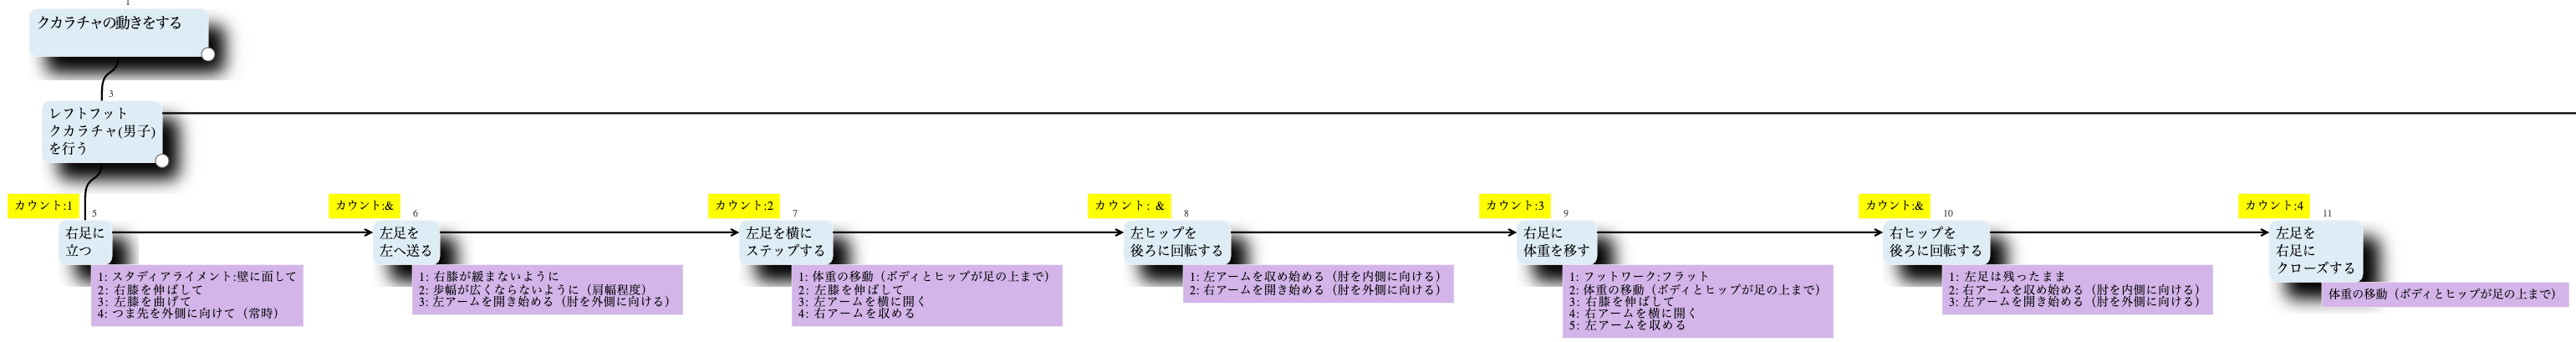
\includegraphics[width=1.0\linewidth]{./image/process_knowledge_instructor1_ver1.png}
    \caption{実験期間中に指導者1によって改良されたプロセス知識}
    \label{fig:process_knowledge_instructor1_ver1}
\end{figure}

指導者2は, この段階では改良を行わなかった. 

\subsubsection{LLMの改良提案を受けての改良}
 次に, 実験終了後にLLMの改良提案を評価した上で, 指導者1がさらなる改良を行った(図\ref{fig:process_knowledge_instructor1_ver2}). この改良では, 上半身の使い方に関するより具体的な指示が追加された. 特に「左足を横にステップする」動作において, 「上半身のストレッチを行う」「ボディとヒップにずれを作る」「左側に上半身を伸ばす」という詳細な指示が加えられた. これはLLMが抽出した「ボディーをストレッチ」という指導コメントに対応する改良であり, 上半身の使い方をより具体的に示すものとなっている. \\

\begin{figure}[htbp]
    \centering
    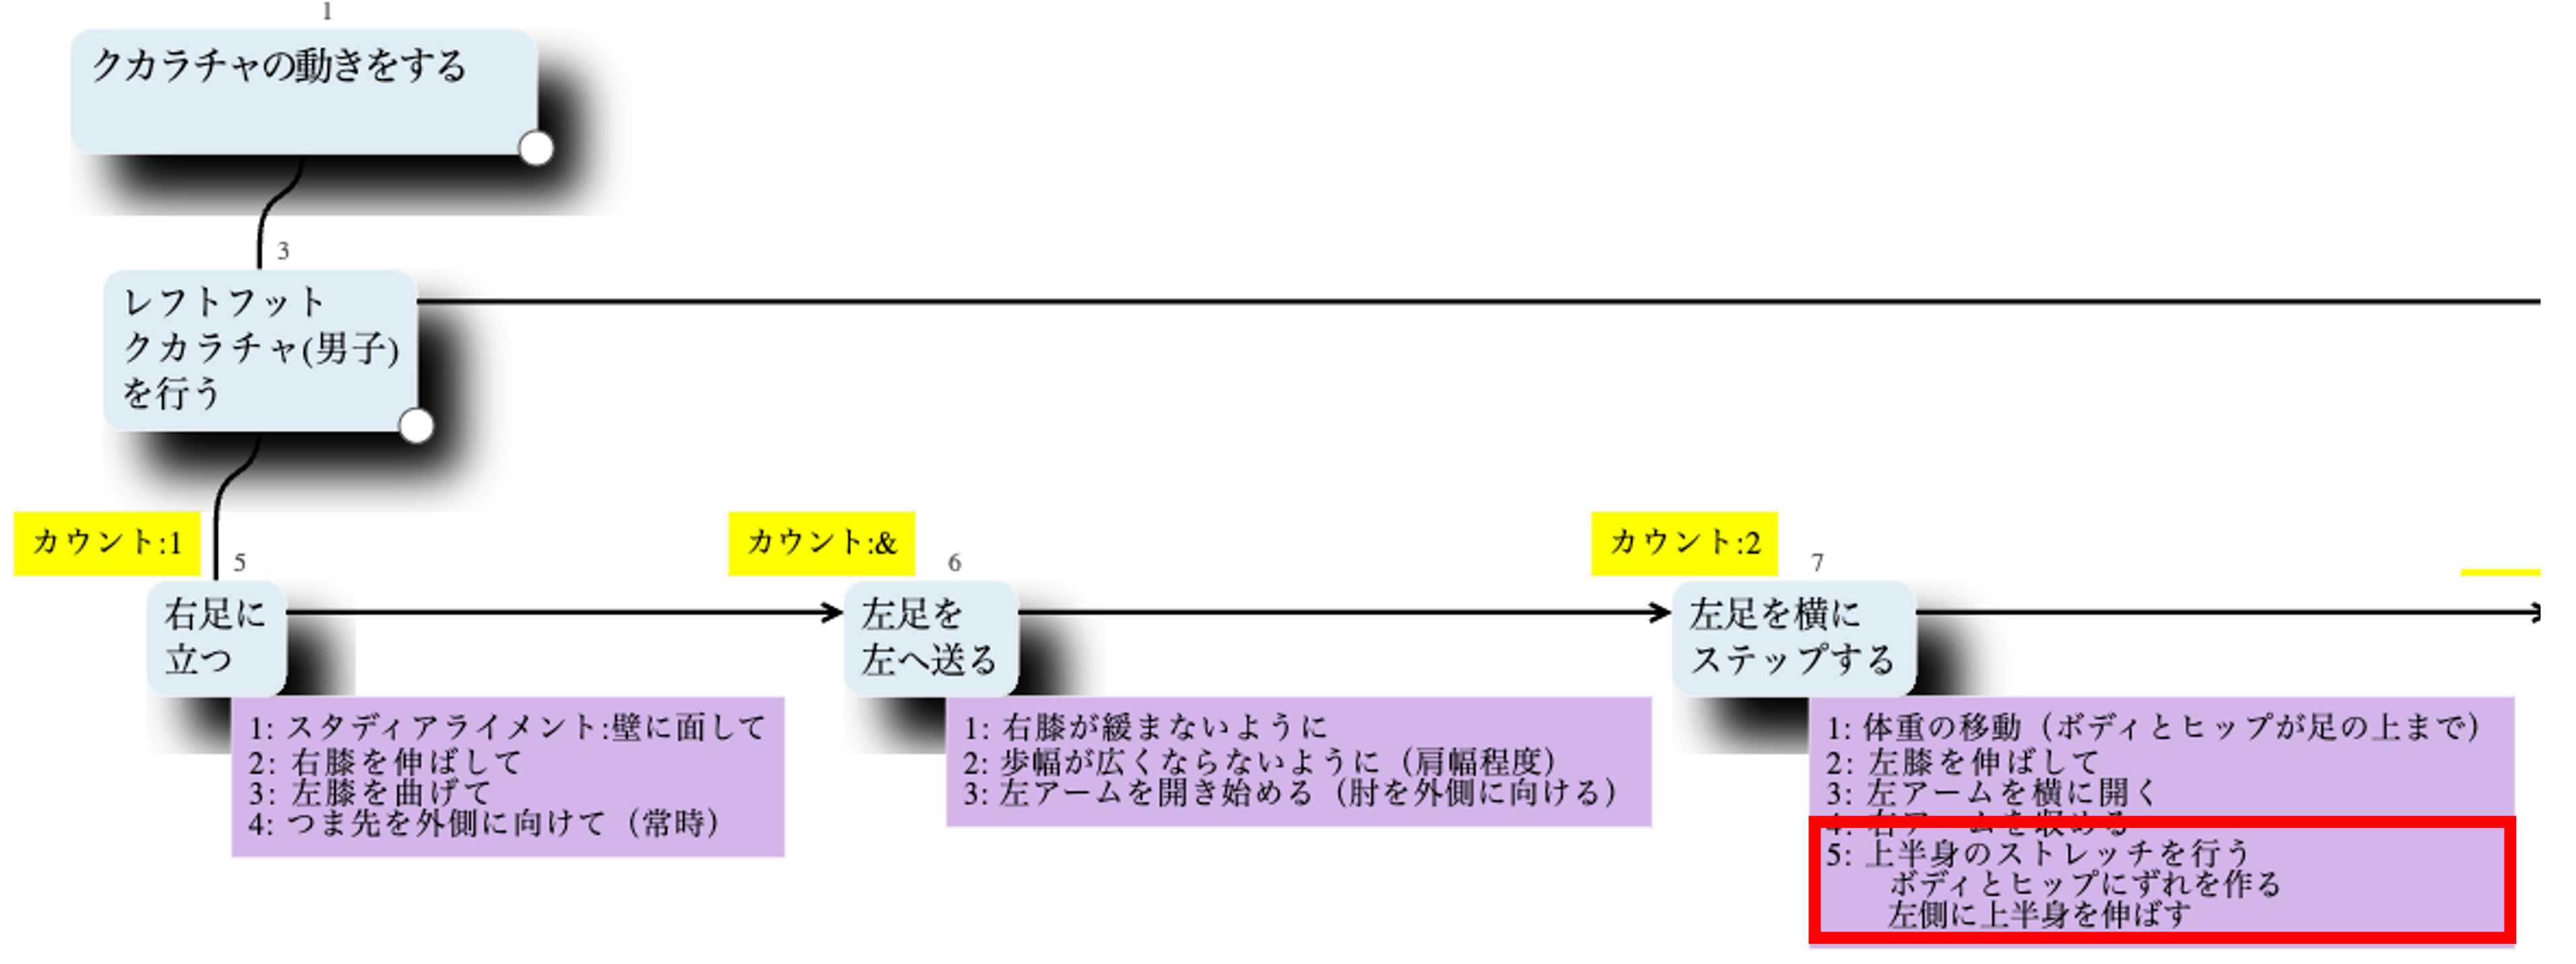
\includegraphics[width=1.0\linewidth]{./image/process_knowledge_instructor1_ver2.png}
    \caption{LLMのフィードバック後に指導者1によって改良されたプロセス知識}
    \label{fig:process_knowledge_instructor1_ver2}
\end{figure}

 一方, 指導者2は特に2つの重要な要素を追加する改良を行った(図\ref{fig:process_knowledge_instructor2_ver1}). 第一に, 「つま先は外側に向ける(継続)」という注意点が動詞の詳細として追加された. これは各動作において常時意識すべき基本的な姿勢要素として位置づけられている. 第二に, 「軸に関して:背骨が上から吊り下がっている感じ, 頭と背骨が床に対して垂直になるイメージ」という軸の保持に関する具体的な説明が追加された. これは抽象的な「軸を保つ」という指示を, より具体的なイメージとして学習者に伝えるものとなっている. \\
 これらの改良の特徴として, 実行タイミング(カウント)や基本的な実行方法(パート・ウェイト, フットワーク等)といった基本的な要素は変更されていない点が挙げられる. 追加された要素は, 動作全体を通じて意識すべき基本的な姿勢や動きの質に関するものであり, 個々の動作の変更ではなく, 動作全体の質を向上させるための指示となっている. これらの改良によって, プロセス知識はより実践的で具体的なものとなり, 学習者がより正確に動作をイメージし, 実行できるようになることが期待される. \\

\begin{figure}[htbp]
    \centering
    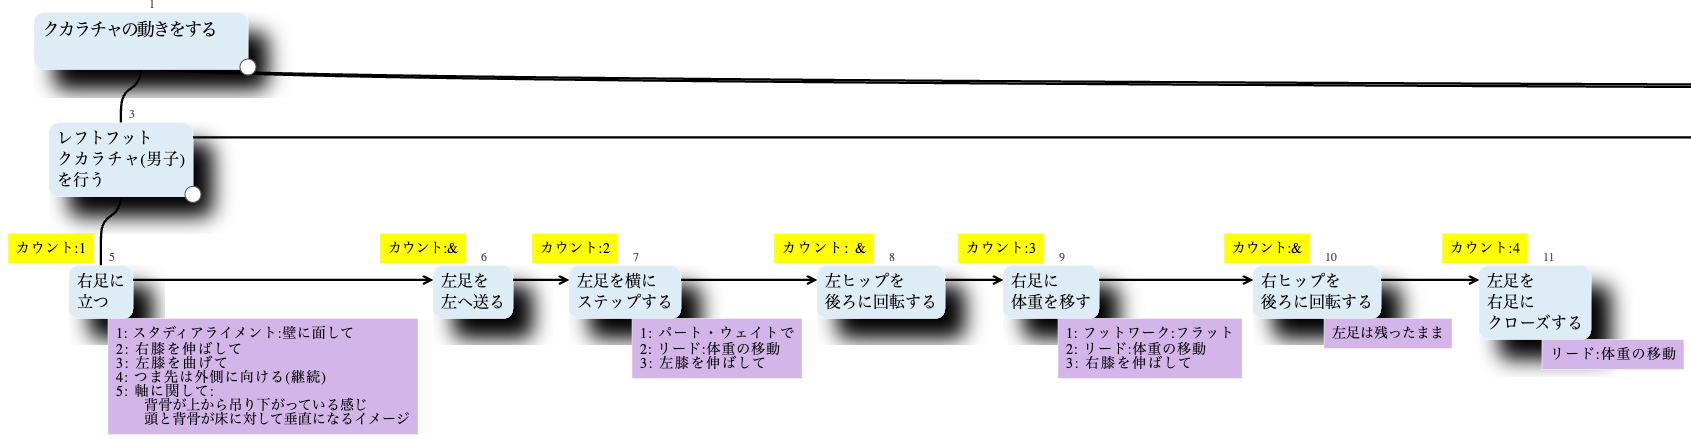
\includegraphics[width=1.0\linewidth]{./image/process_knowledge_instructor2_ver1.png}
    \caption{LLMのフィードバック後に指導者2によって改良されたプロセス知識}
    \label{fig:process_knowledge_instructor2_ver1}
\end{figure}

\subsubsection{提案手法の実現可能性に関する評価}
 プロセス知識の改良結果から, 提案手法が知識抽出・整理の仕組みとして機能することが確認された. これは以下の2つの観点から評価できる.  \\

 第一に, 指導現場での知識抽出が限定的ながら実現されている. 実験期間中, 指導者1は上半身の使い方や体重移動, 歩幅や膝の使い方など, より詳細な動作の質に関する説明を自発的に追加した. これは, 指導活動の中で新たな知識要素を抽出し, それをプロセス知識として形式化できる可能性を示している.  \\

 第二に, LLMの改良提案を介した知識の追加が確認された. 実験終了後, 両指導者はLLMの改良提案を評価した上で, それぞれ異なる観点からプロセス知識を改良している. 指導者1は上半身の使い方に関するより具体的な指示を追加し, 指導者2は姿勢の基本要素に関する詳細な説明を加えた. このことは, LLMを介することで, プロセス知識の改良機会を創出できる可能性を示している.  \\

 一方で持続可能性という観点からは課題が残る結果となった. 実験期間中の自発的な改良は指導者1のみにとどまり, 指導者2は実験終了後のLLMの改良提案を受けてはじめて改良を行った. また, プロセス知識の改良は2回の機会に限定されており, 継続的な改良のサイクルは確認できなかった. このことは, 指導現場での自然な文脈の中で知識抽出・整理の仕組みとして定着させるためには, 自発的な知識抽出を促す仕組みや, より頻繁な改良機会の設定など, さらなる改善が必要であることを示している.  \\

 これらの結果から, 提案手法は指導現場での知識抽出とLLMを活用した知識の追加という2つのアプローチを組み合わせることで, 基本的な知識抽出・整理の仕組みとして機能し得ることが示された. ただし, 持続可能な仕組みとして確立するためには, 特に指導現場での自発的な知識抽出を促進するための改善と, より継続的な改良サイクルを実現するための工夫が必要であると考えられる.  \\

\subsection{学習者による提案手法の受容性評価}
 提案手法が学習者にとって受け入れられ, 効果的な学習支援となり得るかを評価するため, 実験参加者13名中8名(約62\%)からアンケート回答を得た. \\
 回答者の背景として, 全員が週1回以上ダンススタジオで練習を行っていた. 普段の指導内容の理解方法としては, 全員が「積極的に体を動かしながら感覚的に理解する」を選択しており, その他「頭の中で整理しながら理屈で理解する」「レッスン時に先生に質問する」などの方法を組み合わせていた. \\
 システムの利用状況については, 大半の学習者が「レッスン時のみ」の利用にとどまっていた. 利用が限定的だった理由として, 「レッスン時間外にダンスについて考える機会が少なかった」「日常生活が忙しく確認する時間がなかった」「スマートフォンでの操作が面倒だった」などが挙げられた. 一方で, 「先生のコメントを確認するために利用した」「自分の動作や先生のお手本の確認のために利用した」という積極的な利用も一部で見られた. \\
 クカラチャへの理解深化要因については, 「先生からのコメントで理解を深めることができた」という回答が最も多く, 次いで「構造化知識を見ることで理解を深めることができた」「先生の見本動画を見ることで理解を深めることができた」といった回答が得られた. これは提案手法の各要素が学習者の理解促進に一定の効果を持つことを示唆している. \\
 システムに対する要望として, 「大きな画面でもコメントが確認できると良い」「スマートフォンの画面の比率に対応していると学習者が利用しやすい」「コメントが入った時の通知機能があれば良い」といった操作性に関する改善点が指摘された. また「参考資料が比較的少ない」という意見も見られた. 
 これらの結果から, 提案手法は学習者の理解促進に一定の効果を持つことが示された一方で, 日常的な利用を促進するためには, 操作性の改善や通知機能の追加など, より使いやすいインターフェースの実現が必要であることが明らかになった. \\


\section{提案手法の総合的な評価}
 これらの評価結果から, 本研究の目的に対する達成度を以下のように評価することができる. \\
 第一に, 指導現場での知識抽出については, 指導者と学習者の自然な対話から新たな知識要素を抽出することに成功し, その有効性が確認された. 特に, 指導者のコメントの76\%に未含有要素が含まれていたことは, 普段の指導活動の中で知識抽出が可能であることを示している. \\
 第二に, LLMによる知識抽出支援については, 未含有要素の抽出において高い精度(F値0.928)を示し, 知識の体系的な整理に貢献できることが確認された. しかし同時に, 指導の本質的な意図の理解には課題が残ることも明らかになった. \\
 これらの結果は, 本研究が目指したより自然な文脈での知識抽出・整理の仕組みの実現に向けて, 基本的な枠組みは確立できたものの, さらなる改善の余地があることを示している.\\

% 第6章{考察}
\chapter{考察}
・暗黙知を暗黙知のまま伝えること. 形式知化する必要性.\\
・手続き知識の問題点.\\
・オンライン指導の文化の醸成.\\

% 第7章{まとめ}
\chapter{まとめと今後の展望}
 本研究の目的は, 熟練技能者の持つ知識を自然な文脈の中で抽出し, 整理する手法を確立することであった.この目的を達成するため, 本研究では「指導現場での対話収集」と「LLMによる知識抽出支援」を組み合わせた新しい手法を提案し, 社交ダンスを対象とした実証実験を通じてその有効性を検証した.\\
 提案手法の特徴は, 第一に指導現場というワークショップよりも自然に知識が表出する文脈に着目した点にある. 従来の知識発現手法では、ワークショップという特別な場を設定し、意図的な想起と議論に基づいて知識抽出を行う必要があった。これに対し本研究では、指導者と学習者の自然なやり取りの中から知識を抽出することで、より自然な文脈での知識抽出の実現を目指した。第二の特徴は、LLMを知識抽出支援ツールとして活用した点である。これにより、収集された対話から新たな知見を抽出し、それを既存の知識体系に統合していく過程を支援することを試みた。\\
 実証実験では, 石川県内のダンススタジオの協力を得て, 指導者2名と学習者13名による約5週間の実践を通じてデータを収集した. 分析の結果, 以下の点が明らかになった.\\
 第一に, 指導現場での知識抽出の実現可能性が確認された. 収集された指導コメントの76\%に未含有要素が含まれており, 普段の指導活動の中で新たな知識要素を自然に抽出できることが示された. 特に学習者からの質問が, 指導者の暗黙知を引き出すきっかけとなる場面も観察された. また, 同じ技術要素が学習者の状況に応じて多様に表現されるという, 指導現場特有の知識抽出パターンも確認された.\\
 第二に, LLMによる知識抽出支援の有効性が示された. LLMは未含有要素の抽出において高い精度(F値0.928)を示し, 知識の体系的な整理に貢献できることが確認された. ただし, 指導の本質的な意図の理解には限界があり, 人間の専門的な解釈が必要不可欠であることも明らかになった.\\
 さらに重要な発見として, 社交ダンスにおける知識構造の二重性が示唆された. すなわち, 時系列的な動作の連鎖という側面と, その背後にある原理的な知識という側面が存在する可能性がある. この発見に基づき, 技能を「目標層」「原理層」「認知層」「実行層」という4層で捉える分類枠組みと, 実行層の特性による分類枠組みを提案した. これらの枠組みは, 技能分野の特性に応じた適切な知識表現方法の選択に貢献するものである.\\
 特に社交ダンスについては, 時系列的な動作を単層的に記述し, その背後にある原理的な知識をCHARMや目的指向知識の枠組みで表現するという, 二元的なアプローチを提案した. このアプローチは, 社交ダンスに限らず, 同様の特性を持つ他の身体技能分野にも適用できる可能性がある.\\
 本研究の主な貢献は以下の3点にまとめられる.\\
\begin{enumerate}
    \item 自然な文脈での知識抽出の仕組みの提案:\\
    従来のワークショップ形式での知識抽出に代わり, 指導現場での対話とLLMを組み合わせた新しい知識抽出の枠組みを提示した. これにより, より自然な文脈での技能伝承の仕組みの実現可能性を示した.

    \item 身体技能における知識構造の解明:\\
    社交ダンスを事例として, 身体技能における知識構造の二重性を明らかにした. また, この知見に基づいて技能分野を体系的に分類する枠組みを提案し, 技能伝承研究の理論的基盤の拡充に貢献した.

    \item 知識表現方法の選択指針の提示:\\
    技能の特性に応じた適切な知識表現方法の選択指針を示した. 特に, 時系列的な動作記述と原理的な知識記述を分離するという新しいアプローチを提案し, その有効性を示した.
\end{enumerate}
 今後の課題としては, 以下の点が挙げられる.\\
\begin{enumerate}
    \item マルチモーダルなデータ収集・分析の実現:\\
    動作の映像データや非言語情報など, より多角的なデータの収集と分析を行うことで, より豊かな知識体系の構築を目指す必要がある.

    \item LLMの活用方法の高度化:\\
    専門分野に特化した事前学習や, 指導者の意図理解に焦点を当てたプロンプト設計の改善など, LLMの活用方法をさらに発展させる必要がある.

    \item 二元的アプローチの検証と展開:\\
    提案した時系列的動作記述と原理的知識記述の二元的アプローチについて, 実践的な検証を行うとともに, 他の技能分野への展開可能性を探る必要がある.
\end{enumerate}
 これらの課題に取り組むことで, より効果的な技能伝承の実現に向けて研究を発展させる可能性がある.\\


\chapter{謝辞}
xxxxxx

% 参考文献
\renewcommand{\bibname}{参考文献}
\bibliographystyle{custom_style}
\bibliography{Master-paper}


% 付録
%% 付録用の章見出しの設定
\newcommand{\appchapterfmt}{
  \titleformat{\chapter}[hang]
    {\huge\bfseries}
    {付録~\Alph{chapter}\ }
    {0pt}
    {}
}\setcounter{chapter}{0} % 章番号をリセット
\appchapterfmt  % 付録用の章見出しを適用
%% 付録開始
\appendix
\chapter{プロンプト}

\begin{tcolorbox}[breakable, colback=white, colframe=black]
    \begin{minted}{text}

Human:
#概要
「指導コメント」属性と「やりとり情報」属性を参照して「手順構造化データ」の改
良点を指摘してください.

#背景
「what_about」に関する熟練者の暗黙知を引き出します.
そのための方法は以下のような順序で行います.
1.熟練者が対象の動作の手順を階層的に構造化した「手順構造化データ」を用意し
  ます.
2.普段の指導現場で生じるコメントや,やりとりを観察します.
3.観察から「手順構造化データ」に足りない部分を追加したりより適切に表現でき
  る部分を改良します.例えば,指導コメントややりとりでは言及されているのに,
  「手順構造化データ」には含まれていない部分を修正します.

#「手順構造化データ」に関する説明
- 手順構造化データはオントロジーの概念と時系列な手順マニュアルを組み合わせ
  たデータ構造です.
- 上位階層の「行為ノード」はより抽象的であり,下位階層の「行為ノード」はより
  具体的です.
- データの階層は上位階層の「行為ノード」をより詳細に説明することを意味しま
  す.別の言い方をすると,下位階層のデータはその「行為ノード」に含まれるとも
  いえます.
- 階層が深くなるにつれて詳細な説明になっていきます.
- データの順序は時系列を表します.
- 各「行為ノード」には追加の情報が含まれています.


#指示
- 「手順構造化データ」に含まれる「指導コメント」,「やりとり情報」属性を観察
  し,「手順構造化データ」の改良点を提案してください.
- すでに存在する「行為ノード」の改良を提案する場合はどの「行為ノード」を
  改良すればいいか理由とともに明示してください.また,「行為ノード」に付随
  する情報を追加する場合はその属性を明示してください.
- 「行為ノード」の追加を提案する場合は,どの部分に追加すればいいか理由とと
  もに明示してください.追加位置は二つの「行為ノード」を示し,どの「行為ノ
  ード」の間に追加すべきなのか明示してください.
- すでに存在する「行為ノード」の削除を提案する場合はどの「行為ノード」を
  削除すれば良いか理由とともに明示してください.
- 「詳細な注意点」にも従って回答してください.
- 出力は「出力フォーマット」を元にマークダウン形式インデントを利用してわか
  りやすく表現してください.

#詳細な注意点
- 入力された「手順構造化データ」とあなたの提案を比較し, 各階層が同じ抽象度, 
  もしくは同じ具体性を持つような統一された回答をしてください.
- 「行為ノード」の追加を提案する場合は,同じ階層の他の「行為ノード」と言葉や
  粒度感について統一性を持たせてください.例えば,抽象的な「行為ノード」の間
  に具体的な動作を記述することは望ましくありません.その場合は抽象的な「行為
  ノード」を追加した上で,その下位階層に具体的な「行為ノード」を追加してくだ
  さい.
- 「行為ノード」の追加を提案する場合は,階層数を増やしたり減らしたり,ずらし
  たりしたりする提案でも構いません.
- 改良や追加を提案する場合は,「手順構造化データ」が持つ階層構造と時系列構造
  を熟慮してください.
- 階層構造について熟慮すべき点は,あなたの提案がある「行為ノード」の上位概念
  なのか,同じ階層の概念なのか,もしくはより詳細に説明するための下位概念なの
  か等です.
- 時系列構造について熟慮すべき点は,あなたの提案が順番に行う必要がある動作な
  のか, 同時に行う必要がある動作なのかです.
- 動詞の詳細に追記する場合は,それが下位階層の行為ノードとして記述できないか
  検討してください.
- 「指導コメント」と「やりとり情報」に関しては改良や追加, 削除の対象ではあ
  りません.
- その他の提案についてもできるだけ具体的に記述するように心がけてくださ
  い.
- その他の提案ではビジュアライズに関する言及はしないでください.あなたの
  フィードバックは身体動作の手順に関する文脈に限定して使用されます.
- その他の提案では身体動作習得のための学習全体に対する言及はしないでくださ
  い.あなたのフィードバックは身体動作の手順に関する文脈に限定して使用され
  ます.
- あなたが提案する「行為ノード」に関する記述は手順の要素が1つになるように
  してださい.2つ以上の要素が含まれる場合は「行為ノード」を分ける必要があり
  ます.
- 上記全てを提案する必要はありません.「指導コメント」属性や「やりとり情報」
  属性を観察して得られた洞察に基づくことが大事です.
- 特に「手順構造化データ」には含まれていないが,「指導コメント」や「やりとり
  情報」に含まれている情報は熟練者の暗黙知の可能性があり,重要性が高いです.
- あなたのフィードバックを受ける者は必ずしも「手順構造化データ」に精通してい
  るわけではなく,一般的な熟練した指導者である点を考慮し,わかりやすい説明を
  心がけてください.

#出力フォーマット
### 改良点1
```
-改良の種類-

    改良/追加/削除


-改良位置-

    行為ノードのbid:xx
    行為ノードの内容:xx


-改良内容-

    改良内容を記述
```

### 改良点2
```
-改良の種類-

    追加

-改良位置-

    前行為ノードのbid:xx
    前行為ノードの内容:xx
    後行為ノードのbid:oo
    後行為ノードの内容:oo

-改良内容-

    改良内容を記述

```

### 改良点3
```
...
```

### その他の改良提案

    この部分は自由記述

#データの説明
##データの概要
- 「手順構造化データ」は「what_about」の手順を階層的に構造化したもの
  をJSON形式で表現したデータです.
- 手順中の各行為は「行為ノード」として表現され,「data_type」もしくは
 「data_type_name」で判別できます.
- ただし,「text_value」属性が「分岐」の場合は単に階層構造の分岐を表
  していま
  す.
- 下位層の「行為ノード」は上位層の「行為ノード」をさらに詳細に分解した
  ものです.
- 上位層の「行為ノード」は下位層の「行為ノード」を全て満たすことで達成
  されます.
- 同じ階層のノードには順序がある場合と順序がない場合があり,順序の有無は
 「arrow」属性で表され,その順番は「sort」属性で表されます.
- 各「行為ノード」と同じ階層にいくつかの情報が記述されています.これらは
 「行為ノード」に関する追加情報です.この部分に「指導コメント」属性と
 「やりとり情報」属性が含まれています.

##一般的な属性の説明
- charm_head:参照する「手順構造化データ」のタイトルが含まれています.
- charm_data_kinds:「行為ノード」とそれに付随する各種追加情報の
  定義です.
- bid:「行為ノード」のID.
- parent_bid:親ノードのbid.
- sort_no:同じ階層の「行為ノード」における順序.
- arrow:順序の有無.
- charm_branch_datas/charm_branch_data:「行為ノード」やそれ
  に関する追加情報が含まれています.
- childrens:下位層のデータが含まれています.
- data_type/data_type_name:「行為ノード」属性や「指導コメント」
  属性,「やりとり情報」属性等の識別ができます.
  「charm_data_kinds」に含まれる定義と対応します.
- text_value:各属性の内容が記述されています.

##「指導コメント」のデータに関する属性の説明
- 「指導コメント」は「data_type」属性が10,もしくは「data_type
  _name」属性が「指導コメント」のデータです.
- content内には,同じ階層の「data_type_name」が「行為」のデータに
  関連すると判断された「指導コメント」の情報が複数含まれています.
- 「行為」と「指導コメント」の関連性の判断は指導者が行っています.
- annotation_id:「指導コメント」の一意なIDです.「やりとり情報」属性
  とのリレーションを表します.

##「やりとり情報」のデータに関する属性の説明
- 「やりとり情報」は「data_type」属性が11,もしくは「data_type
  _name」属性が「やりとり情報」のデータです.
- chat内には「annotation_id」で示される「指導コメント」に関する
  「やりとり情報」が「指導コメント」別に複数含まれています.ここには
  学習者の質問や感想とそれに対する指導者の回答が記録されています.
- chat_elementsは「発言者:その発言内容」のように表現されたデータ
  が時系列順に含まれています.studentは学習者,teacherは指導者です.


#手順構造化データ
「json_data」

Assistant:
    \end{minted}
\end{tcolorbox}

\begin{comment}

\end{comment}

\end{document}
